\documentclass[12pt]{article}
\usepackage[english]{babel}
\usepackage[utf8]{inputenc}
\usepackage{amsmath}
\usepackage{amssymb}
\usepackage{amsthm}
\usepackage{hyperref}
\usepackage{graphicx}
\usepackage{subcaption}
\usepackage{xcolor}
\usepackage{algorithm}
\usepackage{algpseudocode}
\usepackage{parskip}
\usepackage{afterpage}
\usepackage{mathtools}
\DeclarePairedDelimiter\floor{\lfloor}{\rfloor}
\usepackage{hyperref}
\usepackage{minted}
\usepackage{url}
\usepackage{relsize}





\graphicspath{{figures/}}

\newcommand{\todo}[1]{\textcolor{red}{#1}}

\newcommand{\R}{\mathbb{R}}
\newcommand{\N}{\mathbb{N}}

\newcommand\blankpage{%
    \null
    \thispagestyle{empty}%
    \addtocounter{page}{-1}%
    \newpage}

\newtheorem{theorem}{Theorem}[section]
\newtheorem{corollary}{Corollary}[theorem]
\theoremstyle{definition}
\newtheorem{definition}{Definition}[section]

\title{\textbf{Simulations of Point Processes on Directed Graphs}}
\author{Stavroula Rafailia Vlachou}


\begin{document}
\maketitle
\newpage 
\begin{abstract}
  Simulating a point process where the events correspond to vehicle collisions on a road network can be quite computationally heavy due to the large number of elements that are necessary to provide a sufficient discretization of the network. This paper aims to present a computationally efficient solution for simulating events of a point process. With this goal in mind, an end to end application is developed that starts by constructing a discretization of the road graph to represent the state space of the process and associating accidents with elements of the road graph, and goes on to simulate events of the process from one or more realisations. The simulation of events is done in a two-level approach; first the arrival times are obtained via inversion and then the incidents are located on the graph by sampling from the conditional distribution of the states given the arrival times. Even though the state space is constructed from hundreds of thousands of edges and vertices, the application is relatively efficient in terms of computing time and given enough compute nodes in a distributed computing framework is able to scale to arbitrarily large state spaces. Future work shall revolve around a finer partitioning of the road network and the incorporation of additional characteristics of the events, under a marked point process. 

\end{abstract}
\begin{center}
    \textbf{Keywords:} Spatial Data Analysis, Point Processes, Simulations, Road Networks, Road Graphs, OpenStreetMap, Apache Spark, Spatial Partitioning  
\end{center}
\newpage
%\blankpage

\tableofcontents
\newpage 

\section{Introduction} 
The rise of automated driving systems (ADSs) and their incorporation in commercial vehicles gives rise to a demand for a safety protocol for these systems. For an automated system to be adopted by society, an evaluation not only of the performance, but also of the risk that the system imposes should be conducted and ADSs are no exception. In the case of ADSs, the evaluation of risk is of high importance since these driving systems fall under the category of \emph{safety critical systems}. The term refers to these systems whose failure or malfunction can cause physical harm to the individuals involved. The risk evaluation of an ADS system can be decomposed into two aspects; ``the probability of occurrence of harm and the extent of that harm"\cite{risk}. Thus, a measure of the probability of system malfunction or failure that results in some kind of harm is necessary. In addition, according to risk tolerability principles, such as GAMAB (Globalement Au Moins Aussi Bon), meaning ``in total at least as good", the risk of a new system should not exceed the risk of existing systems that serve similar purposes \cite{riskGAME}. 
Thus, a first step towards such a measure is to compare that probability with the respective probability that a human operator imposes. To do so, extensive simulations need to be performed on different driving scenarios that include specific conditions, such as the weather and light conditions, the time of day, the type of road, etc. 
 
This project amounts to the modelling of vehicle collisions as events of an underlying point process whose state space is a mathematical formalism of a physical road network, as a road graph. Effort is made to simulate further events of the process in the most efficient way possible, under the scope that it would be beneficial to help quantify the risk of the human driver. 

Lastly, it is hoped that this work will be a contributing step towards setting the stage for answering the following safety related questions:

\textit{What is the risk of a human driver given a spatio-temporal position?}

\textit{For a given time what is the risk of an accident occurring in a specific road segment?}


\section{Data Availability and Collection}
\subsection{Accident Records Dataset}\label{AccidentRecordsdata set}
The first dataset utilised in this work consists of $11991$ records of traffic collisions documented in Lithuania during a four year period from $2017$ to $2020$. These records are restricted to accidents that resulted in death or injury of some kind that befell the individuals involved. Accidents where no physical harm to individuals is recorded are stored in a separate database for insurance purposes. 

The accident dataset was queried from a relational database consisting of four interrelated tables provided by the company Sensmetry. The database itself was initially acquired as part of the Common Accident Data Set (CADAS) database. CADAS is a European Commission initiative that amounts to a database consisting of accident records in a uniform format among European countries. This uniform format allows for data compatibility and comparison regardless of the national data collection system and consists of a minimum set of standardised data elements \cite{CADAS}. In addition, one of the main advantages that comes along with this uniform format is that any framework built for a dataset extracted from CADAS can process any other dataset from the database, regardless of the country in which the initial records are collected from. Consequently, this allows for a generic application that is country-agnostic and can potentially be used for processing any European country's vehicle collision data that enforces the CADAS template.  

Within the CADAS framework the variables are structured into four categories; Accident, Road, Traffic Unit and Person where each category corresponds to a relational table in the database. In total, there are $64$ attributes that describe several characteristics of an event, such as, weather and lighting conditions, geographic location and the model of the vehicle. For the purposes of this work the focus is on the geographic location in terms of latitude and longitude and the date-time of the accident. These are attributes of the Accident and Road categories. With this in mind, the provided database was queried and the desired variables were obtained from each table. These variables, together with the accident id variable, were then merged into a single table. Consequently, the retrieved dataset used for the rest of this work consists of the following attributes; 

\begin{minted}{python}
  a1_id, r1_latitude, r2_longitude, a2_date, a3_time
\end{minted}

The accident id is a unique identifier of a record in the initial database and acts as a primary key of the four tables. The latitude and longitude fields correspond to the recorded coordinates of each event measured in the national coordinate system of Lithuania (LKS94). These coordinates were assigned by the responding police officer on the scene of each accident. The last two variables, as their names indicates, refer to the calendar date and time of day that the collision took place.

\subsection{Road Network Datasets} \label{RoadNetworkdataSets}
In order to implement any kind of spatial analysis that revolves around events on the road one needs to obtain a dataset that corresponds to a discretization of the underlying road network. The most natural discretization of a road network is based on it's core element: roads. In addition, the dataset of accident records described in section \ref{AccidentRecordsdata set}, is restricted to incidents taking place within Lithuanian boarders. As a result, the appropriate road network to associate this data with is the Lithuanian one. Fortunately, little effort is needed in obtaining such a dataset due to OpenStreetMap (OSM)\cite{OpenStreetMap}; an open source collaborative project that provides a database of geographic data. The data for the road network of Lithuania was retrieved from OSM through Geofabrik GmbH\footnote{\url{http://geofabrik.de}} \cite{GeoFabrikLT}; a server that provides extracts from the OpenStreetMap project. The obtained file was formatted under the Protocol Buffer Binary format (PBF); a format developed by Google in order to serialise structured data in a language and platform neutral manner \cite{PBF}.  

OpenStreetMap structures the data on four topological primitives: \textit{nodes}, \textit{ways}, \textit{relations} and \textit{tags}. \textit{Nodes} are essentially geographic points whose position is described by latitude-longitude pairs measured in the World Geodetic System $1984$ (WGS$84$). These \textit{nodes} are used to define \textit{ways} which are lists of ordered \textit{nodes} and are frequently used to model linear features, such as roads or rivers. The last two core elements of OSM are firstly, \textit{relations}, which are used to represent the relationship between \textit{nodes} and \textit{ways}, and \textit{tags} that are used for storing metadata. Regarding the \textit{tags} that are associated with roads, OSM has a long list of \textit{tags} that can be used to describe the type of road, e.g.\texttildelow motorway or pedestrian. From the road-type specific \textit{tags} documented by OSM, a subset was extracted in an attempt to filter out roads that vehicles cannot enter. For example, the \textit{tag} with value ``footway" was excluded since it is used to describe roads that are exclusively used by pedestrians and thus no vehicle can enter. However, it should be emphasised that the list is not exhaustive and should be adapted according to the desired granularity and level of road importance relevant to the analysis at hand.


The \textit{tags} used for this analysis and their description, as provided by OSM, \footnote{\url{https://wiki.openstreetmap.org/wiki/Map_features}, retrieved on $12/05/2022$} are summarised below:
\begin{itemize}\label{tags}
    \item \textbf{motorway:} A restricted access major divided highway, normally with $2$ or more running lanes plus emergency hard shoulder.
    \item \textbf{motorway{\_}link:} Roads leading to/from a motorway.
    \item \textbf{trunk:} The most important roads in a country's system that aren't motor\textit{ways}.
    \item \textbf{trunk{\_}link:} The link roads leading to/from a trunk road from/to a trunk road or lower class highway.
    \item \textbf{primary:} The next most important roads in a country's system. (Often link larger towns.) 
   \item \textbf{primary{\_}link:} Roads leading to/from a primary road from/to a primary road or lower class highway.
   \item \textbf{secondary:} The next most important roads in a country's system. (Often link towns.)
   \item \textbf{secondary{\_}link:} Roads leading to/from a secondary road from/to a secondary road or lower class highway.
   \item \textbf{tertiary:} The next most important roads in a country's system. (Often link smaller towns and villages)
   \item \textbf{tertiary{\_}link:} Roads leading to/from a tertiary road from/to a tertiary road or lower class highway.
   \item \textbf{living{\_}street:} For living streets, which are residential streets where pedestrians have legal priority over cars, speeds are kept very low and where children are allowed to play on the street.
   \item \textbf{residential:} Roads which serve as an access to housing, without function of connecting settlements. Often lined with housing.
   \item \textbf{road:} A road/street/motorway/etc.\texttildelow of unknown type.
   \item \textbf{construction:} Roads under construction.
   \item \textbf{motorway{\_}junction:} Indicates a junction (UK) or exit (US).
   
\end{itemize}

From a geographic point of view the Lithuanian road network is present in OSM by $21212155$ \textit{nodes}, with $1299907$ of them structured in $137540$ \textit{ways}. Within the road network the \textit{node} dataset is limited to those \textit{nodes} that belong to at least one \textit{way}, among the \textit{ways} that have one of the \textit{tags} from the chosen subset of \textit{tags} described previously. As a result, \textit{nodes} that represent buildings, parks, residencies, etc.\texttildelow are not included. The final number of distinct \textit{nodes} is $162325$.   

\begin{figure}[!ht]
    \centering
    \subfloat[\centering Accidents in Lithuania ($2017-2020$) ]{{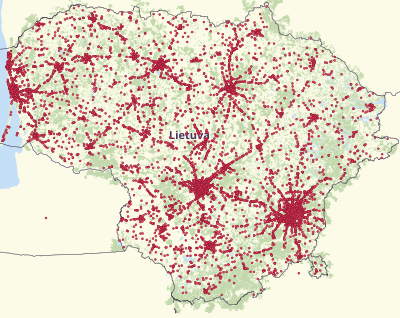
\includegraphics[width=6.70cm]{images/LTall.png} }}%
    \qquad
    \subfloat[\centering Accidents in Vilnius ($2017-2020$) ]{{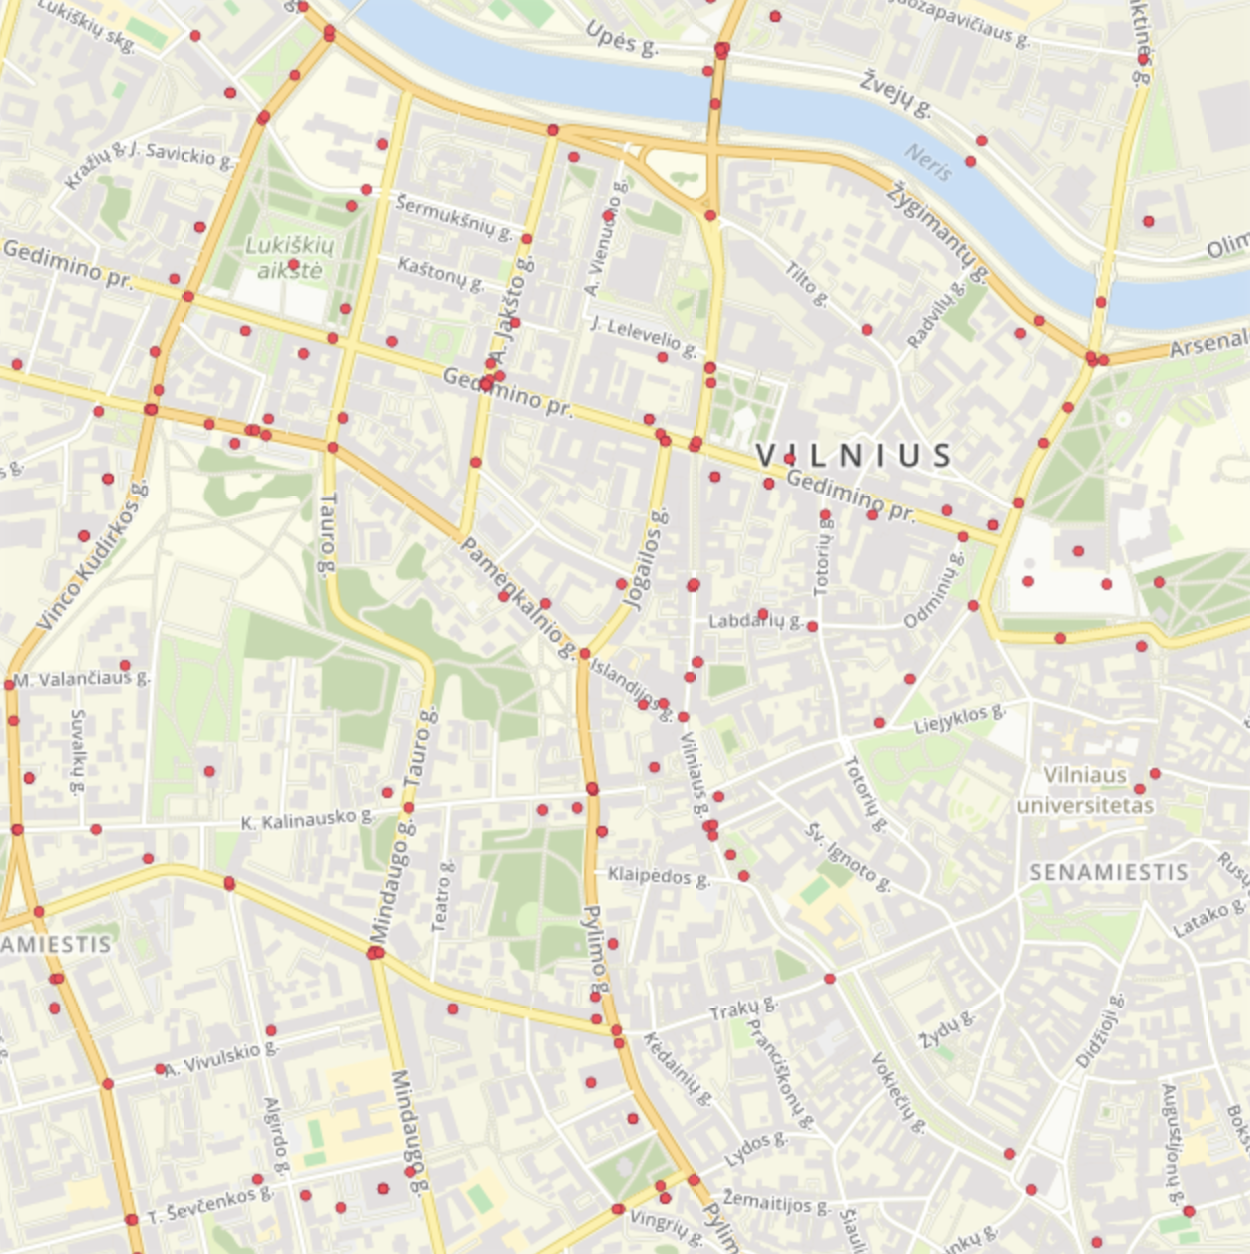
\includegraphics[width=5.30cm]{images/Vilnius.png} }}%
    \caption{Accidents in Lithuania and the country's road network over the four year period $2017-2020$. (a) All of the recorded accidents in Lithuania. Note the formed clusters in urban centres. (b) Accidents that occurred in a small area in the centre of the capital Vilnius and the underlying road network.}%
    \label{fig:AccidentsOSMmap}
\end{figure}
Figure \ref{fig:AccidentsOSMmap} provides a visualisation of the accidents recorded throughout the four year period in Lithuania, where the documented accidents are shown as red points. On the left, all available accidents are mapped in terms of geographic location within the country's borders. Note the clusters formed around cities; a result to be expected since traffic intensity is increased in urban areas and as a result these areas could be characterised as being more accident-prone. On the right of Figure \ref{fig:AccidentsOSMmap} a small area in the capital Vilnius is shown, were the underlying road network of the city is also visible. It is worth noticing, that the location of some points does not lie exactly on any road but rather in close proximity to one. This, indicates the necessity of associating such points with an element of the road network.


\section{Data Ingestion, Validation \& Processing}\label{ingestion}
Towards ingesting the accident dataset in a distributed computing environment, validating each one of the attributes for all records and further processing of the data, a Scala library was build. From an ingestion point of view, the library consists of four parser functions; one for each table. Apart from loading the files, these functions implement a set of validation tests for every single record according to a specified schema that the data should be compliant with. Non-valid values are flagged for further inspection. Lastly, the library wraps some additional functions for geospatial processing. It is worth mentioning that the ingestion of all $11991$ records and the validation of all $64$ attributes (i.e. $11991\times 64$ values in total) is completed within a couple of seconds on a system with CPU of $8$ cores and $16$ GB of memory.  
\subsection{Data Ingestion}
The first step towards the ingestion of the data is done by the two main parser functions on the Accident and Road tables. After the obtained dataset described in Section \ref{AccidentRecordsdata set} is loaded, the validated dataset is structured according to the parquet format. Apache Parquet \footnote{\url{https://parquet.apache.org}, retrieved on $12/05/2022$
} is an open source implementation inspired by Dremel \cite{dremelPaper} for an efficient, language-agnostic, compressed and binary file format where each file is organised by column, rather by row. The latter allows for smaller storage space and faster run-time for analytical queries. In addition, the parquet files of the data are used in order to obtain the data files in delta format, which can be understood as parquet files with key-value properties for storing metadata. The delta format has the following properties; Atomicity, Consistency, Isolation and Durability (usually referred to as ACID properties), which ensure the accuracy and integrity of the data, even in the event of a failure \cite{deltaPaper}. Moreover, delta files allow for quick and accurate data updates and removal of records which makes them compliant with the General Data Protection Regulation (GDPR) \footnote{\url{https://delta.io}, retrieved on $12/05/2022$}. Lastly, both formats of the data files are integrated into the distributed file system of a deployed Apache Spark cluster, to allow further processing and geospatial queries.  

For the ingestion of the entire OSM Lithuanian road network dataset, the PBF file obtained from OSM is transformed to three parquet files; one for each primitive (\textit{nodes}, \textit{ways} and \textit{relations}), by utilising methods of the osm-parquetizer project \footnote{\url{https://github.com/adrianulbona/osm-parquetizer}}. The first two generated files, corresponding to the \textit{nodes} and \textit{ways} data are then transferred into the distributed file system for further exploitation.  


\subsection{Data Validation and Quality}\label{DataValidationAndQuality}
To elaborate on the validation that takes place at the ingestion level, the focus is shifted on the set of validation rules and how these rules are obtained. Looking at the metadata of the CADAS database, one is able to establish a set of syntactic rules regarding the possible values that each attribute value can take. These syntactic rules allow for a first validation process of the data to ensure that all of the values are compliant with the predefined schema. Testing each record against these syntactic rules is the first step taken towards establishing the validity of the dataset and ensuring that unreasonable values are filtered out. 

The next step towards data validation is logical or semantic validation. Taking into account that there is no way of validating the time and date, the validation for those is restricted to the time attribute taking values from the $24-$ hour clock and the date corresponding to any valid calendar date of the given year. While validating the time attribute values, $9$ records were assigned the value $9999$ as the time of day that the corresponding accident occurred. This value is used throughout the database as a flag, meaning that the respective value is unknown. These records of unknown time were not excluded from the dataset as for this work the lowest time resolution is chosen to be the day of the year. Having established that, the semantic validation is shifted towards the recorded location of the accident.

The bounding box of Lithuania is used as a first measure of location validity. Since the analysis is restricted to Lithuanian territory, coordinate values that do not belong to a region of Lithuania are marked as non-valid. Through this process $37$ non-valid coordinates were found and communicated back to the Lithuanian Transport Agency for revision. Fortunately, $35$ out of $37$ location measurements were revised and their values were reassigned, contributing towards an increase of the quality of the database. The exact location of two accidents is not accurately known and thus these two records are excluded from the analysis. After the validation that occurred within the ingestion process, the number of accident records is $11989$. In addition, since the focus is on events that fall on the road network, accident locations that are not on the road network and not within a certain radius from a point of it are also disregarded (described in detail in Section \ref{MapMatchingPointsOnARoadGraph}). 

Regarding the road network data obtained by OSM, one has to take into account that the project is created by volunteering users, not in a top-down approach but rather from the individual's initiative and thus the quality and completeness of measurements is not guaranteed. Many attempts have been made in order to systematically analyse the quality of the OSM data, with the majority of them concluding that the quality of OSM diverges with location. Haklay \cite{HAKLAY} compares the road network representation of England in OSM with its respective one in the Ordance Survey UK Meridian 2 dataset, in terms of its positional accuracy, and describes the OSM extract ``as a good representation in terms of positional accuracy", while emphasising ``serious issues about completeness". Zielstra and Zipf \cite{zielstra} in their comparative study among the German OSM data and the TeleAtlas MultiNet data, note that the ``coverage of OSM in rural areas is too small", while ``in larger cities the data diversity is so rich that already projects that are based on proprietary data are being replaced with OpenStreetMap data". Despite such limitations, OSM is used because it is openly available unlike proprietary maps available from Vendors. Moreover, OSM data is improvable at least in principle through voluntary activities.  

\subsection{Data Pre-Processing}\label{DataPreProcessing}
In order to be able to relate and analyse the accident events dataset and the road network dataset within the same country-agnostic framework, a uniform spatial reference system is required for the two datasets. However, as previously mentioned, the location of the accident events is expressed in coordinate pairs of latitude and longitude measured in meters according to the national coordinate system of Lithuania (LKS94). At the same time, OSM data are expressed in the unit of decimal degrees according to the World Geodesic System (WGS84). Taking into account that the volume of the road network dataset is significantly larger than the accidents dataset, and that the WGS84 coordinate system is perhaps the most widely used spatial reference system globally (when the unit of measure is degrees), the coordinates of the accident events were projected on that system. 

For parts of the analysis such as the map-matching described in section \ref{MapMatchingPointsOnARoadGraph}, both datasets were projected to the Lambert Azimuthal Equal-Area (ETRS89) coordinate reference system \footnote{usually referred to as European Grid}. The choice of this system is justified by the fact that the map-matching algorithm considered here makes use of coordinates expressed in meters in order to calculate distances among them. At the same time, the European Grid allows for some flexibility in processing the accident datasets of any European country, as it covers all countries within Europe and it is recommended for the purposes of statistical analysis from the European Commission \cite{3035}.

To summarise, after pre-processing there are two versions of each dataset in terms of coordinates; one in which the unit of measure is the meter and one where coordinates are expressed in their equivalent values in decimal degrees. 

\section{Road Graph}\label{RoadGraph}
So far, the term road network has been intuitively used to describe the OpenStreetMap representation through \textit{nodes} and \textit{ways} that are associated with a list of road specific \textit{tags}. To give some formalism, a definition of a road network is provided below.

\begin{definition}[Road Network]
    A road network is defined as $\mathcal{N}(N, W)$, comprising a set of points $N=\{n_1, n_2,...,n_k\}$ as \textit{nodes} that are connected amongst themselves by the set of directed road segments $W=\{w_1, w_2,...,w_{k'}\}$ as its links \cite{roadNetworkDef}.
\end{definition}

For this work, the road segments mentioned in the above definition are assumed to be a subset of the OSM \textit{ways}.

\begin{definition}[Intersection]
    Given a road network $\mathcal{N}(N, W)$ the set of intersection points $\mathcal{I}$ is defined as the set of points that lie in at least two road segments $w_i, w_j\in W$ for $i\neq j$. 
    \begin{equation*}
        \mathcal{I} = \bigcup_{i,j,i\neq j} \{w_i\cap w_j\}
    \end{equation*} for $w_i, w_j\in W$. 
\end{definition} 

In order to give a more mathematical representation of the road network, the latter is transformed into a graph, which for the rest of this work shall be referred to as road graph. Before that, the definition of a graph is provided together with the relevant notation.

\begin{definition}[Graph]
    A graph is a pair $G=(V,E)$ such that $E\subseteq V^2$; thus the elements of $E$ are $2-$ elements (pairs) of $V$. The elements of $V$ are the vertices of the graph $G$ and the elements of $E$ are the edges of $G$. \cite{GraphDef}
\end{definition}

The vertex set of a graph $G$ is referred to as $V(G)$, while its edge set as $E(G)$.

The number of vertices of a graph $G$ is its order, written as $|G|$, and its number of edges is denoted by $||G||$.

\begin{definition}[Road Graph]
    A road graph is a graph $G(V,E) $ constructed based on some spatial partitioning of a road network $\mathcal{N}(N, W)$.
\end{definition}  

\subsection{Construction of a Road Graph}\label{ConstructionOfARoadGraph}
Different approaches have been used to create a road graph out of a road network depending on the elements of the network that are to be analysed. Anwar, Liu, Vu and Leckie \cite{roadNetworkDef} in their work towards studying the trade-off between accuracy and efficiency of different strategies, adopt a density peak partitioning strategy. From this view point, the road network is partitioned based on traffic measures and the similarity of the measures among different sub-networks. Despite the impressive results, this traffic-based approach yields a great complexity that can be avoided since the focus of this work is around the topology of the road network rather than a partitioning in sub-networks of similar traffic patterns. 

For the construction of a road graph $G(V,E)$ there are several topological partitioning schemes of the road network $\mathcal{N}(N,W)$ that can be followed and it is the partitioning scheme at hand that controls the complexity (in terms of number of edges and vertices) of the final road graph. The simplest case of spatial partitioning is to consider each point $n\in N$ as a vertex $v\in V$ and to connect the resulting vertices according to the road network structure given by the road segments of $W$. Despite its simplicity, this approach results in a road graph where the number of vertices is equal to the number of points on the road network, i.e. $|V(G)|=|N|$; and this number can easily explode if the point representation of the real urban network is too rich or the road network itself corresponds to a large urban area. 

Another partitioning strategy is to restrict the set of points of the road network by only considering points that correspond to intersections or dead end points. Then, each intersection or dead end point is mapped into a vertex, and vertices that correspond to points of the same road segment $w\in W$ are connected with edges. This approach significantly reduces the number of vertices $|V(G)|$ of the graph, while keeping most of the information regarding the structure of the network. Pseudo-code to construct a road graph from a road network following the latter partitioning strategy is presented in Algorithm \ref{alg:G0}. The road graph constructed by Algorithm \ref{alg:G0} is going to be referred to from now on as $G_0$ and it is the baseline model of the project. The vertices of $G_0$ correspond to intersections or dead end points, while the edges represent the road segments between these points.  



\begin{algorithm}
  \caption{Constructing a Road Graph from a Road Network}
  \label{alg:G0}
  \begin{algorithmic}
    \State{\textbf{Input:} Road Network}
    \Procedure{RoadGraph}{$\mathcal{N}(N,W)$}
    \State $V \gets \emptyset$
    \Comment{Initialisation}
    \State $E \gets \emptyset$
    \For{$way \in W$}
    \State \({V_{way}\gets []}\)
        \For{\(node \in way\)}
            \If{node is Intersection or Dead End}
            \State \(V_{way} \gets V_{way} ++ \{node\}\)
            \Comment{Create and append vertex}
            \EndIf
        \EndFor
    \For{i=0 until $||V_{way}||-2$}
    \State{\(v_i\gets V_{way}[i]\)}
    \Comment{Element of $V_{way}$ at position $i$}
    \State{\(v_{i+1}\gets V_{way}[i+1]\)}
    \State \(E \gets E \cup edge(v_i, v_{i+1})\)
    \Comment{Create edge}
    \EndFor
    \State {$V \gets V \cup V_{way}$}
    \Comment{Global vertices from all ways}
    \EndFor
    \State {$G_0 = (V,E)$}
    \Comment{Create graph}
    \State \textbf{return} {$G_0$}
    \EndProcedure
    \State{\textbf{Output:} Road Graph}
  \end{algorithmic}
\end{algorithm}

\begin{figure}
    \centering
    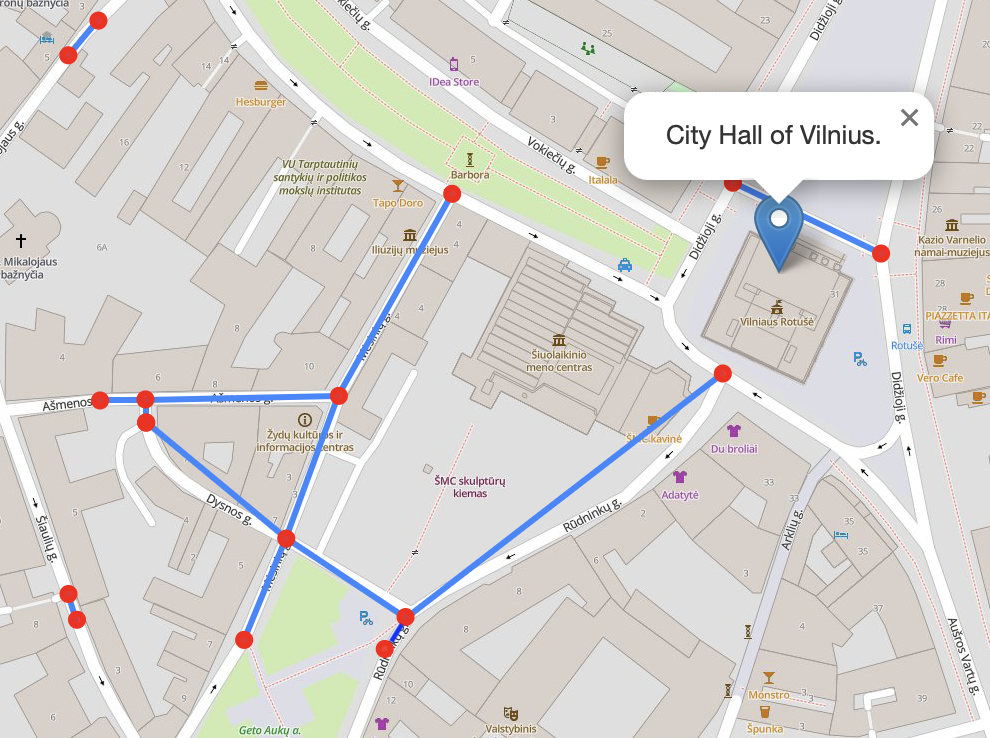
\includegraphics[width=11cm]{images/G0.png}
    \caption{The road graph $G_0$ for a small area around the City Hall of Vilnius. The vertices are represented by red points, while the edges among them with blue lines.}
    \label{fig:G0}
\end{figure}

Figure \ref{fig:G0} illustrates the baseline road graph $G_0$ constructed for a small area surrounding the City Hall of Vilnius. The vertices of the graph, where in this case corresponding to intersection points or dead ends are represented by red points. It is worth mentioning that in the graph of Figure \ref{fig:G0} vertices can be seen where there is no obvious intersection or dead end point. The reason behind this is that, these points mark the end of the road segments in the bounded road network dataset that was extracted for the purposes of this visualisation. Having said that, the edges connecting vertices that belong to the same road segment or different road segments via their common intersection points, are visualised by blue lines. The initial road network consists of $1243$ \textit{nodes}, with $36$ of them structured in $14$ \textit{ways}. Among these \textit{nodes}, $5$ of them belong to at least $2$ \textit{ways} resulting to $5$ intersection points. From this road network, the road graph was constructed by Algorithm \ref{alg:G0} and the result consists of $16$ vertices associated  with $13$ edges. As can be seen in the illustration of the graph, there are some roads around the City Hall that are not present it the constructed graph. The reason behind this has to do with the type of road they are classified as and more specifically with the \textit{tag} associated with them in their representation as \textit{ways} in OSM. Specifically in this case, the roads in the exact perimeter of the City Hall have a \textit{tag} of value ``unclassified". This \textit{tag}, counter intuitively with the word, does not mean that the classification is unknown, but is rather used for roads whose importance belongs to the lowest level possible in a country's system. The ``unclassified" \textit{tag} is not among those used in the set of \textit{tags} (described in Section \ref{tags}) chosen for this work and as a result, the $ways$ with this \textit{tag} are not present in the discretization of the network.  

\begin{figure}
    \centering
    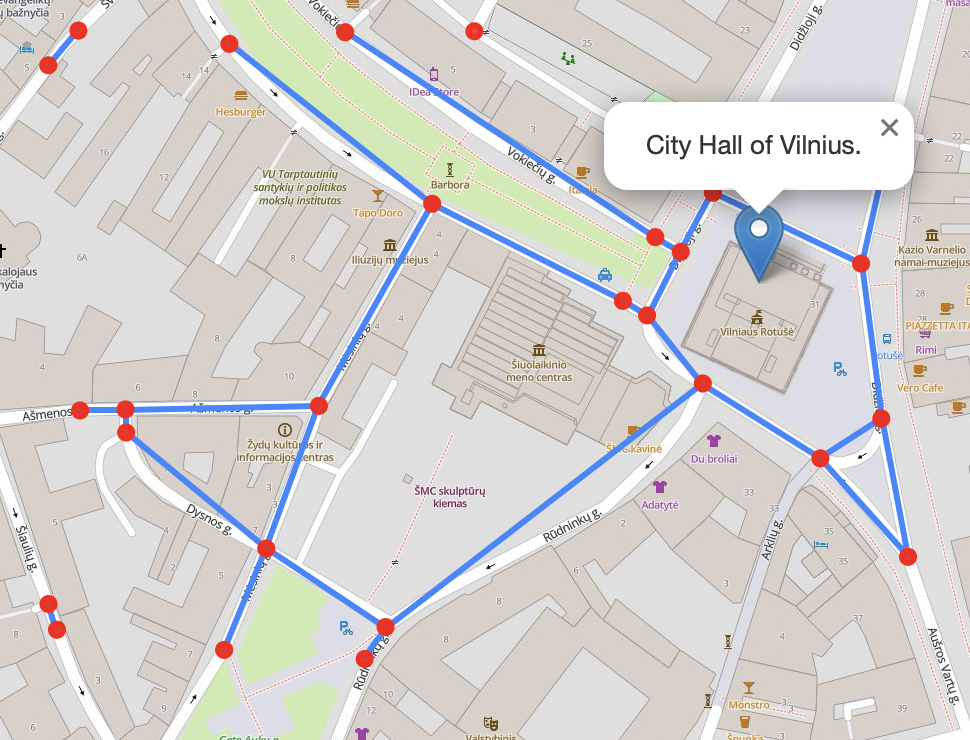
\includegraphics[width=11cm]{images/G0Unclassified.png}
    \caption{The road graph $G_0^*$ for a small area around the City Hall of the capital Vilnius, from a more rich road network that includes roads of the lowest importance within the road network. The vertices are represented by red points, while the edges among them with blue lines.}
    \label{fig:G0Unclassified}
\end{figure}

For illustration purposes only, the ``unclassified" \textit{tag} was included in an attempt to showcase the idea behind Algorithm \ref{alg:G0} for this small area of Vilnius. The new graph constructed from the less restricted set of \textit{ways} is shown in Figure \ref{fig:G0Unclassified}. Looking at Figure \ref{fig:G0Unclassified}, one can see that for all of the intersection and dead-end points present in the area, as well as the road segment among those, vertices and edges are created constituting a graph that preserves the real structure of the road network. Emphasis should be put in the fact that \textit{ways} labelled as ``unclassified" are not used for the rest of this work. 

\begin{algorithm}
  \caption{Constructing a weighted road graph from a road network}
  \label{alg:G0Weighted}
  \begin{algorithmic}
    \State{\textbf{Input: \textit{ways} of a road network}}
    \Procedure{WeightedRoadGraph}{W}
    \State $V \gets \emptyset$
    \Comment{Initialisation}
    \State $E' \gets \emptyset$
    \For{$way \in W$}
    \State \({V_{way}\gets []}\)
        \For{\(node \in way\)}
            \If{node is Intersection or DeadEnd}
            \State \(V_{way} \gets V_{way} ++ \{node\}\)
            \Comment{Create and append vertex}
            \EndIf
    \EndFor
    \State \(distance \gets 0\)
    \Comment{Initialisation}
    \State {$node \gets way[0]$} \Comment{First element of the way}
    \For{i=1 until $||way||-1$}
        \If{$way[i] \in V_{way}$}
        \State \(E' \gets E' \cup edge(node, way[i], distance)\)
        \Comment{Weighted edges}
        \State \(distance \gets 0\)
        \Else 
        \Comment{Accumulate distances}
        \State $distance \gets distance + dist(node, way[i])$
        \State \(node \gets way[i]\)
        \EndIf
    
    \EndFor
    \State {$V \gets V \cup V_{way}$}
    \EndFor
    \State {$G_0' = (V,E')$}
    \State {\textbf{return} {$G_0'$}}
    \EndProcedure
    \State{\textbf{Output:} Road Graph with distance weights}
  \end{algorithmic}
\end{algorithm}

Algorithm \ref{alg:G0Weighted} is an extension of Algorithm \ref{alg:G0} which results in a weighted road graph $G_0'$, while following the same partitioning strategy of only considering intersections and dead end points as vertices. The weights of $G_0'$ are edge attributes that correspond to an approximation of the geodesic distance between the two vertices of each edge. What is worth mentioning is that, in order to calculate the distance as accurately as possible, given the available points on the road network, the cumulative distance of all intermediate points in the road segment at hand is taken into account (instead of considering only the geodesic distance among the two vertices). 

The graph obtained by implementing Algorithm \ref{alg:G0Weighted} provides a good mathematical representation of the road network for urban centres, since in those areas intersection points are found quite frequently in close distance from one another. However, in cases when the road network expands to a whole country's urban infrastructure, $G_0$ suffers from sparse vertices whose corresponding points on the road graph lie at a very large distance from one another. An example of such case is a highway which typically expands over hundreds of kilometers and the only intersection points on the highway are very few entrance or exit points from and to local roads. In other words, the vertices of $G_0'$ are points within a relatively small distance when those vertices correspond to points in a city or a town and a very large distance when the points on the road network are within rural areas. Thus, in order to enable the control of distances among vertices on $G_0$, a distance threshold should be taken into account. According to that threshold, a new vertex is created whenever the desired distance is met. This way, the level of segmentation of the road network can be controlled by the distance threshold and consequently obtain a more rich partition of the network. Based on this partition a new graph is constructed where edges connect points on a \textit{way} such that their distance does not exceed a specified value. The algorithm for partitioning the weighted road graph $G_0'$ and constructing the re partitioned graph $G_1$ is shown in Algorithm \ref{alg:G1partitioned} in pseudo-code. 

\begin{algorithm}
  \caption{Coarsening a Weighted Road Graph}
  \label{alg:G1partitioned}
  \begin{algorithmic}
    \State{\textbf{Input:} Weighted Road Graph, \textit{way}, distance tolerance}
    \Procedure{Coarsen}{$G_0'(V,E'),way,max\_distance$}
    \For{$edge \in E'$}
        \If{$edge.distance > max\_distance$}
        \State{$E'\gets E'\setminus edge$}
        \Comment{Remove edge}
        \State {$previous\_node \gets way[0]$}
        \State{$previous\_src \gets egde.src$}
        \State{$d \gets 0$}
        \For{$i=1$ until $||way||-1$}
            \State{$node\gets way[i]$}
            \If{$d>max\_distance$}
            \State{$V \gets V ++ \{previous\_node\}$}
            \Comment{Create new vertex}
            \State{$edge \gets edge(previous\_src, previous\_node, previous\_distance)$}
            \State{$E' \gets E'\cup \{edge\}$}
            \State{$d\gets d - previous\_distance$}
            \Comment{Remaining distance}
            \State{$previous\_src = previous\_node$}
            \Else
            \State{$previous\_distance \gets d$}
            \Comment{Current distance}
            \State{$d\gets d + distance(previous\_node, node)$}
            \Comment{Accumulate distance}
            \EndIf
            \State{$previous\_node\gets node$}
        \EndFor
        \State{$edge \gets edge(previous\_src, edge.dst)$}
        \State{$E'\gets E'\cup \{edge\}$}    
            
        \EndIf
    \EndFor    
    \State{$V_{new}\gets V$}
    \State{$E_{new}\gets E'$}
    \State {$G_1 = (V_{new},E_{new})$}
    \State {\textbf{return} {$G_1$}}
    \EndProcedure
    \State{\textbf{Output:} Coarsened Weighted Road Graph}
  \end{algorithmic}
\end{algorithm}


An example of such a further partitioning and the relevant graph created by Algorithm \ref{alg:G1partitioned} is given in the visualisation of Figure \ref{fig:WeightedAndCoarsened}. In this case the distance threshold is set to be $100$ meters and thus each edge connecting vertices whose distance is greater than $100$ is split until the desired proximity is achieved. In the weighted road graph for the small area around the City Hall there is one edge connecting two vertices whose approximated distance is $141$ meters. Implementing Algorithm \ref{alg:G1partitioned} results in another weighted road graph for that area, where the suffering edge is removed and replaced by two additional edges. These edges connect each vertex of the initial edge with an intermediate point in the \textit{way} of the road network that they both lie in. Both of the new edge's weights are now less than $100$ meters and their sum equals to the weight of the removed edge. In the visualisation, the intermediate vertex is coloured in green and the removed edge is represented by the dashed black line. Lastly, all of the edge weights for both graphs are represented by the numerical values in black next to each edge/line. 

\begin{figure}[!ht]
    \centering
    \subfloat[\centering Weighted Road Graph  ]{{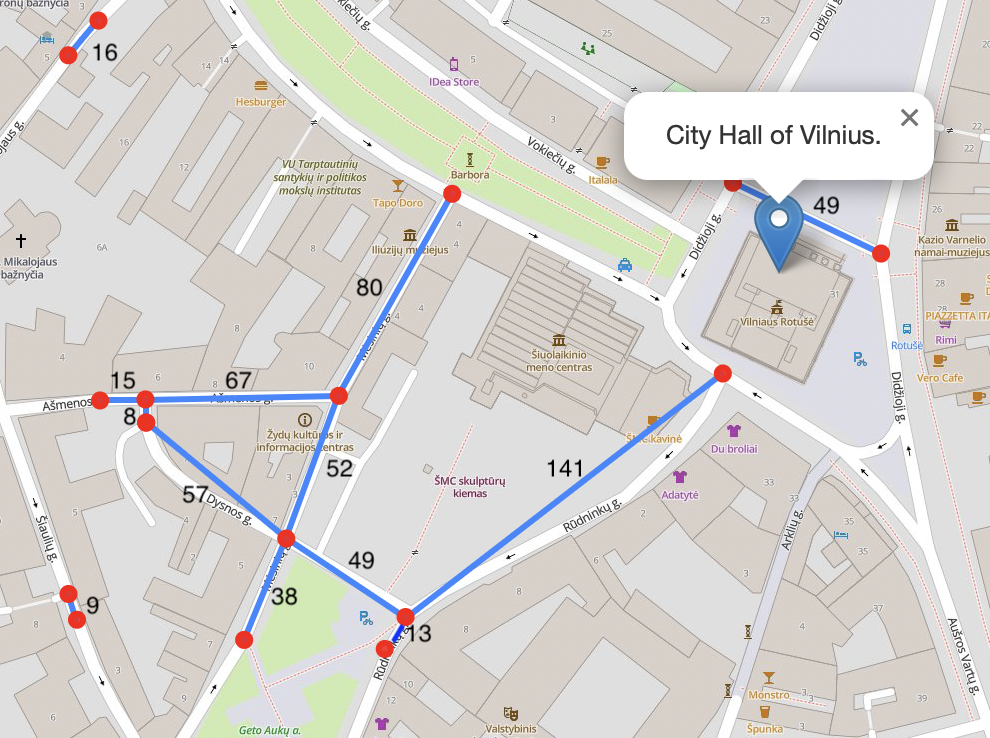
\includegraphics[width=8.5cm]{images/G0W.png} }}%
    \qquad
    \subfloat[\centering Coarsened Road Graph   ]{{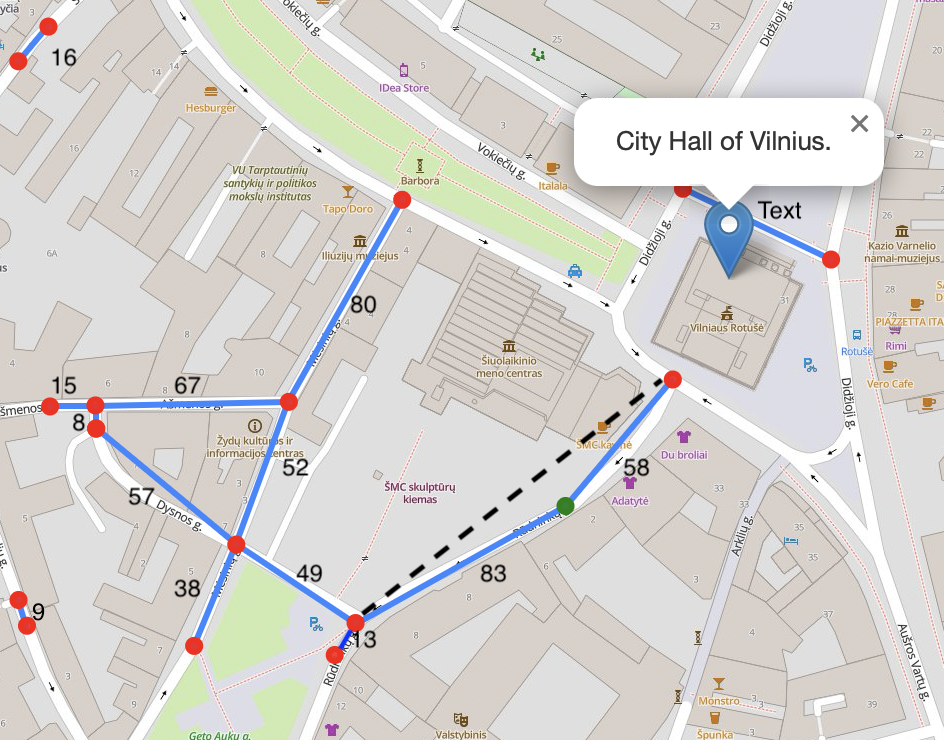
\includegraphics[width=8.5cm]{images/G1.png} }}%
    \caption{The weighted road graph and the coarsened road graph based on a distance of tolerance $100$ meters for a small area around the City Hall of Vilnius}%
    \label{fig:WeightedAndCoarsened}
\end{figure}

Let $\mathcal{N}_{LT}(N,W)$ be the road network obtained for Lithuania from the dataset described in Section \ref{RoadNetworkdataSets}. Then, $|N|=162325$, $|W|=137540$ and $|\mathcal{I}|=162325$. Implementing Algorithm \ref{alg:G0} on $\mathcal{N}_{LT}(N,W)$ results in a road graph $G_{0_{LT}}$ with $191991$ vertices and $237069$ edges, i.e. $||G_{0_{LT}}||=191991$ and $|G_{0_{LT}}|=237069$. It is worth noting that the set of edges $E(G_{0_{LT}})$ has a significantly larger number of elements than the set of vertices $V(G_{0_{LT}})$, which indicates that a great proportion of vertices have degree greater than one. The bar plot of Figure \ref{fig:degrees} depicts the number of vertices aggregated by their degree on the graph. As can be seen from the Figure, the majority of vertices participate in at least $2$ edges, while only a small proportion of vertices (around $15\%$) are a part of a single edge. 

Using the baseline graph of Lithuania $G_{0_{LT}}$ in Algorithm \ref{alg:G0Weighted} returns a weighted road graph $G_{0_{LT}}'$ with the same number of vertices and edges. By inspecting the weights of $G_{0_{LT}}'$ while considering a distance tolerance of $100$ meters, $137207$ edge weights exceeding the distance tolerance are identified. The corresponding edges should be split into smaller edges whose weight is within the defined tolerance. To do so, Algorithm \ref{alg:G1partitioned} is implemented and the returned road graph $G_{1_{LT}}$ consists of $685121$ vertices and $734682$ edges. 

\begin{figure}
    \centering
    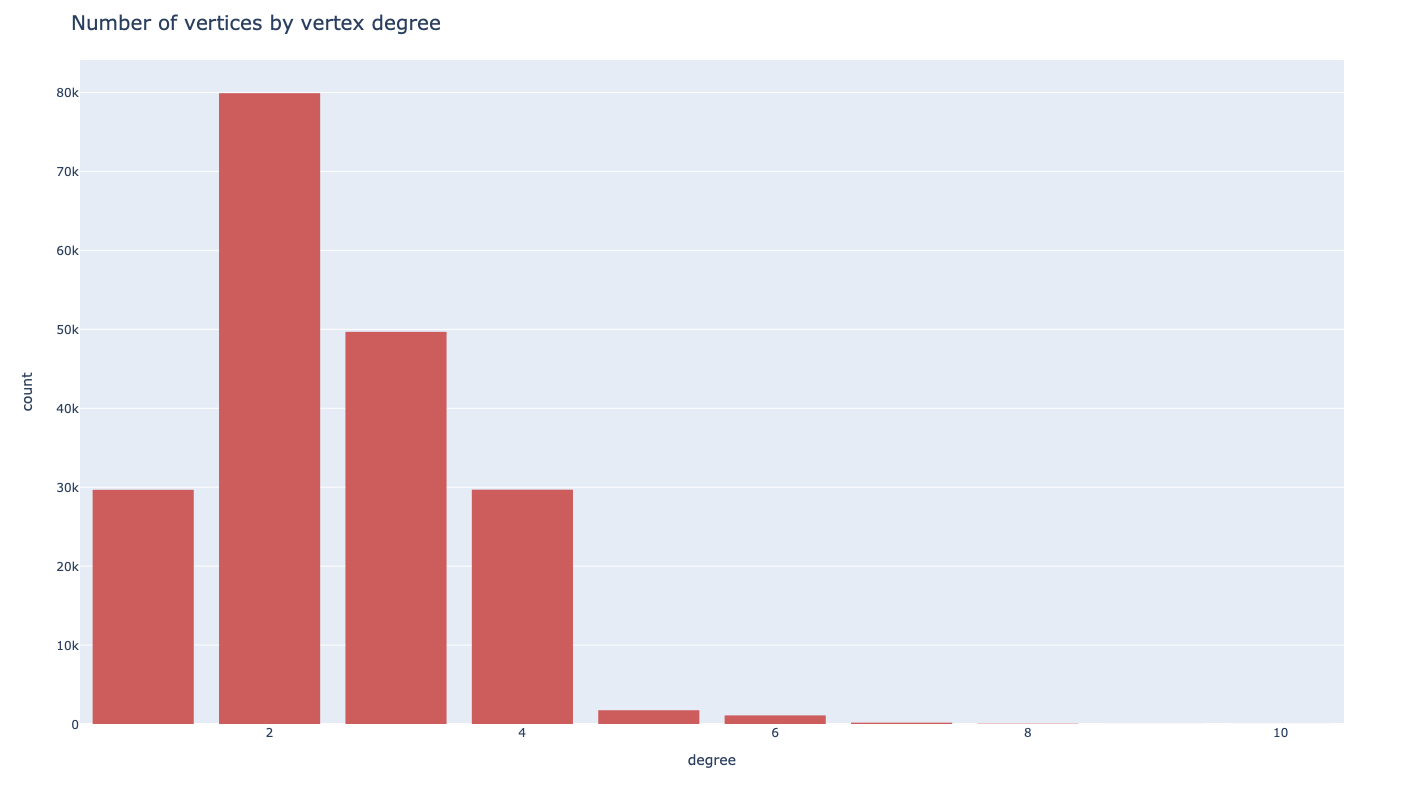
\includegraphics[width=13.5cm]{images/degreeDistribution.png}
    \caption{The number of vertices of the road graph $G_0$ aggregated by the vertex degree.}
    \label{fig:degrees}
\end{figure}

\section{Map-Matching Points on a Road Graph}\label{MapMatchingPointsOnARoadGraph}
\subsection{Background}
Map-matching is an essential procedure in any kind of spatial analysis since it allows for points that do not belong to a spatial structure such as a road network or a road graph to be mapped into elements of the structure. There are many ways to implement the mapping but the most simple and widely used one is to match points based on their geographic location through the nearest available distance. Taking into account that the road network at hand can be arbitrarily large, since it corresponds to a whole country's road network, the associated road graph has a significant number of vertices and edges. As a result, the demand for a highly efficient and scalable map-matching algorithm rises. GeoMatch \footnote{\url{https://github.com/bdilab/GeoMatch}} is a map-matching data pipeline implemented within the Apache Spark ecosystem which distinguishes itself among other applications due to its simplicity, efficiency and suitability for big data and large scale map-matching. Notably, in a comparative study with other state-of-the-art map-matching frameworks such as Megallan, LocationSpark, and GeoSpark, GeoMatch outperformed the rest of the frameworks not only in terms of run-time but also in processing accuracy, achieving almost $97.5\%$ \cite{GeoMatch}.

GeoMatch's performance gains are mainly subject to its data partitioning strategy. The latter is based on Hilbert space-filling curves and an optimal grouping of data based on the generated Hilbert indexes. 

\begin{definition}[Space-Filling Curve]
    A space-filling curve is a curve whose range contains the entire $2$-dimensional unit square (or more generally, an $n$-dimensional unit hyper cube). A Hilbert space-filling curve is a special type of space-filling curve that is constructed as the limit of a sequence of piece wise linear curves. The $n^{th}$ element - curve of the sequence has length $2^n-\frac{1}{2^n}$ and consequently although each curve is contained within the unit square, the length grows exponentially with $n$. 
\end{definition} 

What is worth mentioning is that Hilbert space-filling curves can also be implemented efficiently in cases where the data points do not lie in a square \cite{HilbertNonSquare}. 

The partitioning scheme deployed in GeoMatch is crucial since it is often the case with spatial data that the majority of points are concentrated along few urban areas. Thus, while it is important to keep spatially close data points among the same partition, it is of equal significance to have load balancing among partitions. 

The GeoMatch pipeline takes as input two datasets; the first dataset consists of a set of poly-lines (a sequence of points, essentially a road segment in this context), while the second dataset is a set of points that are to be matched (expressed as GPS coordinates). The first step of the algorithm is the spatial indexing of the data and their allocation among the available processing units. The partitioning schema is built based on both datasets, instead of sampling. Specifically, spatially close indexes are assigned in the same partition while distributing the load fairly among the partitions. Once the partitions are populated a tree-structure is constructed by the road segments in an attempt to reduce the time for the spatial query and avoid a full-search of all possible matches. Next, for each point a spatial query is made in order to retrieve the $k-$ nearest neighbours. To increase the accuracy of the match the distance between the point and the candidate poly-lines is calculated and the match is rejected if the distance is greater than a predefined distance threshold. The output of the pipeline is the second dataset with each point matched with a list of poly-lines of the first dataset. Notably, the result consists of all of the elements of the second dataset, including points with no matched found. This is an important detail since this way, all of the dataset of points that are to be map-matched is carried through the pipeline enabling further processing.

Pseudo-code for the main steps of the GeoMatch algorithm is provided in Algorithm \ref{alg:MapMatching}. 

\begin{algorithm}
  \caption{Map-Matching a point to its $k$-nearest polylines}
  \label{alg:MapMatching}
  \begin{algorithmic}
    \State{\textbf{Input:}Points, PolyLines, $max\_distance$}
    \Procedure{GeoMatch}{Points, PolyLines}
        \Procedure{HilbertIndexes}{Points, PolyLines}
        \State{Compute the Hilbert indexes}
        \EndProcedure
    \State {Group spatially close indexes}
        \Procedure{RTree}{PolyLines}
        \State{Generate R-tree of PolyLines}
        \EndProcedure
        \Procedure{SpatialQuery}{Point, $k$, R-tree}
        \State{Match each point with $k$ candidate PolyLines}
        \EndProcedure
    \For{match $\in$ (point, candidates)}
      \If {distance(point, candidate) $< max\_distance$}
      \State{$Match \gets Success$}
      \Else 
      \State{$Match \gets Reject$}
      \EndIf
    \EndFor  
    \EndProcedure
    \State{\textbf{Output}:Points and their $k$ nearest PolyLines}
  \end{algorithmic}
\end{algorithm}

\subsection{Implementation}
Since the interest lies on events occurring on the road network, the map-matching in this work is to be done in a way that each event is matched with an element of the road graph. Thus, map-matching amounts to associating each recorded event to a vertex or an edge of the road graph. In addition, taking into account that the events correspond to accidents on the road we are especially interested in intersection points and the area within a small distance from such points. 

In this work the implementation of the map-matching algorithm is done in a two-level approach. In the first level all of the events are matched against all intersection points of the road network (which is a subset of the vertices $V$ of the graph), while in the second one all of the events for which no match is found in the first iteration are matched against the road segments (edges $E$ of the graph). During the first round of map-matching $3743$ events out of $11989$ are found to have their $1-$ nearest neighbours within a small distance (that was set to $20$ meters) from an intersection point. Then, the remaining $8246$ points are matched against the road segments by identifying their nearest edge on the road graph. Finally, after the second round of the map-matching algorithm $269$ points are found not to have a nearest neighbour within $200$ meters and are thus omitted from the dataset. This results to a final dataset of accidents consisting of $11720$ data points. 

Regarding the configuration parameters, the dimension of the Hilbert space-filling curve is set to its default value $256$, while the distance threshold above which a match is rejected is set to $20$ meters for the first iteration of the algorithm (where the points are matched against the intersection points) and $200$ meters for the second iteration (where the remaining points are matched against the road segments). One thing to note is that, the number of successful matches highly relies on the configuration of the parameters, since if for example the maximum distance is set to a very small number no match will be found apart for those points which are located on the road network and consequently the $1-$ nearest neighbour is the point itself (with distance $0$). 

Lastly, a technical detail worth mentioning is that the algorithm takes as input coordinates measured in decimal degrees and thus all involved coordinates are re projected into the European Grid coordinate system. 
 
 \begin{figure}[!ht]
    \centering
    \subfloat[\centering Before Map-Matching ]{{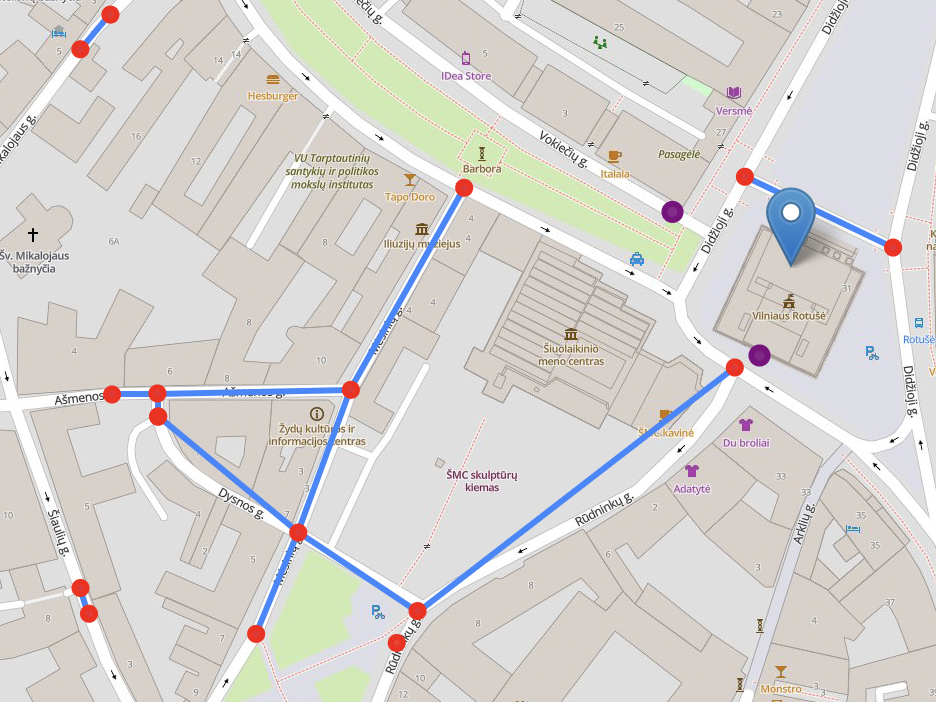
\includegraphics[width=8.5cm]{images/BeforeMapMatching.png} }}%
    \qquad
    \subfloat[\centering After Map-Matching  ]{{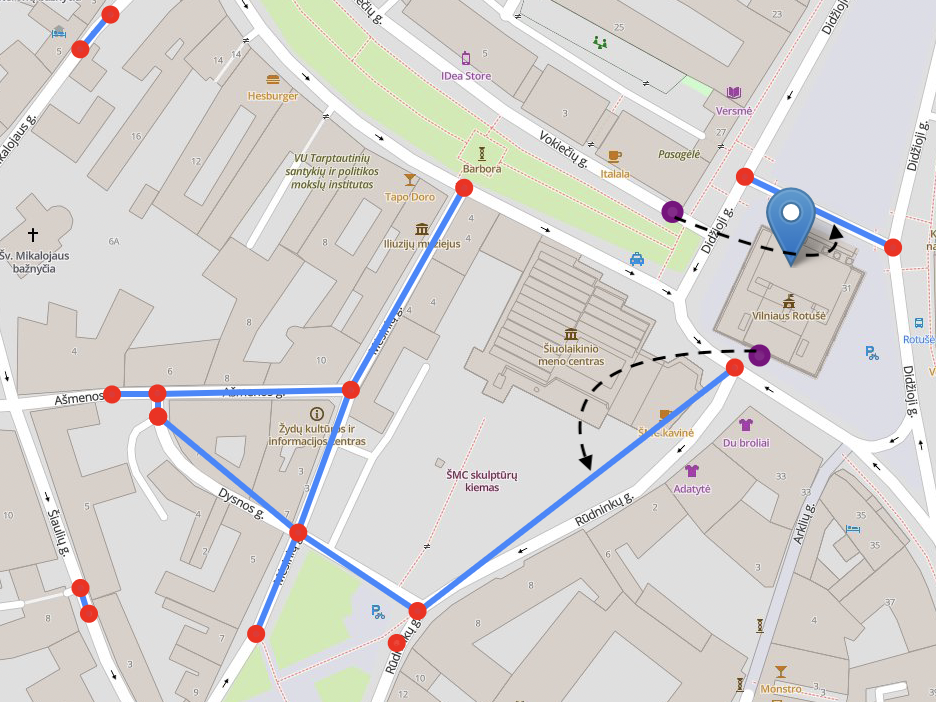
\includegraphics[width=8.5cm]{images/AfterMapMatching.png} }}%
    \caption{Map-matching with GeoMatch on a road graph. The recorded accidents for that area are shown as purple points. (a) Before map-matching the accidents do not lie in an element of the road graph. (b) After the map-matching each accident is associated with one edge of the road graph. The connection is illustrated by the black curved arrows.}%
    \label{fig:MapMatching}
\end{figure}

In the two plots of Figure \ref{fig:MapMatching} one can see the recorded accidents for that area as purple points and the road graph for the small area in Vilnius, before and after the implementation of the map-matching. Looking at the illustration before the map-matching, there are two accidents falling into the area of focus that do not belong in one of the vertices or edges of the road graph. During the map-matching, the $1$-nearest neighbours for these points are found and after the procedure is complete both points are related to an edge of the graph. This relation is presented in the Figure by the curved arrows pointing from the accident point to their $1$-nearest edge. 

After the implementation of the map-matching Algorithm \ref{alg:MapMatching} on the road graph, each point of the accident dataset is matched against one edge or one vertex of the graph. This way, by aggregating the edges and the vertices, each one of them is related with a list of points that are from now on considered to have occurred on those edges or vertices. On the same note, each edge and vertex of the graph is marked by an integer that indicates the total number of accidents that happened on those. Furthermore, if the graph elements are aggregated additionally by the day of the year, the per day number of accidents on each vertex and edge is obtained.

\section{Poisson Process}
\subsection{Mathematical Background}
\begin{definition}[Point Process]
    A point process is a collection of points randomly allocated to intervals of the real line, rectangles or hyper-rectangles in a d-dimensional Euclidean space \cite{daleyPointProcess}.
\end{definition}

One of the most popular point processes, is the Poisson point process which is often used to model the arrival of random, independent events.

\begin{definition}[Poisson Point Process]
    Let $\mathcal{X}$ be a complete separable metric space, $\mathcal{B}(\mathcal{X})$ be the Borel $\sigma-$ algebra generated by the open spheres of $\mathcal{X}$ and $N(A)$ be the number of points in a bounded set $A\in \mathcal{B}(\mathcal{X})$. The Poisson process can be defined, under the assumption that there exists a bounded finite Borel measure $\Lambda(\cdot)$ such that, for every finite family of disjoint bounded Borel sets $\{A_i, i=1,...,k\}$
    \begin{equation}\label{PoissonAbstract}
        P\{N(A)=n_i, i=1,...,k\} = \prod_{i=1}^k\frac{[\Lambda(A_i)]^{n_i}}{n_i!}
    \end{equation}
    The measure $\Lambda(\dot)$ is called the parameter measure of the process. 
\end{definition} 

Embedded in the above definition are the following properties:
\begin{enumerate}
    \item The number of points in each set $A$ has a Poisson distribution.
    \item The number of points in disjoint sets $A_i, A_j \forall i\neq j, i,j\in\{1,...,k\}$ are independent random variables. 
    \item The distributions are stationary, meaning that they depend only on the volume of the set $A$.
\end{enumerate}

For $\mathcal{X}=\mathbb{R}$ the above definition can be used to specify the Poisson process on the real line. Specifically, for $\Lambda(A)=\lambda l(A)$\footnote{$l(\cdot)$ denotes the Lebesgue measure} for some constant $\lambda$, the homogeneous Poisson process on the real line is obtained, while for $\Lambda(A)=\int_A \lambda(x)dx$ the Poisson point process is characterised as non-homogeneous (or in-homogeneous).

In cases where the arrival times of events in a system vary significantly over time, the non-homogeneous Poisson process (NHPP) can be used to model the occurrences of these events. In such a case, the cumulative intensity function is 
\begin{equation}
    \Lambda(t) = \int_0^t \lambda(\tau)d\tau 
\end{equation}
and can be interpreted as the expected number of events in the system by time $t$. In this work the NHPP is used to model the occurrence of accidents falling on the road graph since the number of accidents recorded for each day of the four year period varies not only day by day but also hour by hour within the same day. However, for this work the lowest time resolution of interest is the day of the year and for each day the total number of accidents that occurred is known. In addition, taking into account that the days of a year are discrete while a Poisson process is defined on a continuous domain (here the real line), each day of the four year period is assigned an integer value that corresponds to the $i^{th}$ day of the period, starting from $01-01-2017$, which is mapped to the value $1$. In other words the time horizon of the Poisson process is restricted to the interval $(0, 1461]$, where the value $1461$ is interpreted as $31-12-2020$ and one unit of time is set to be one calendar day. This way, the empirical cumulative intensity function of the NHPP is known for each integer value $i\in \{0,...,1461\}$. The latter indicates that the cumulative intensity could be estimated for any time $t\in (0,1461]$ if a reasonable interpolation between the known values is utilised. 

\begin{figure}
    \centering
    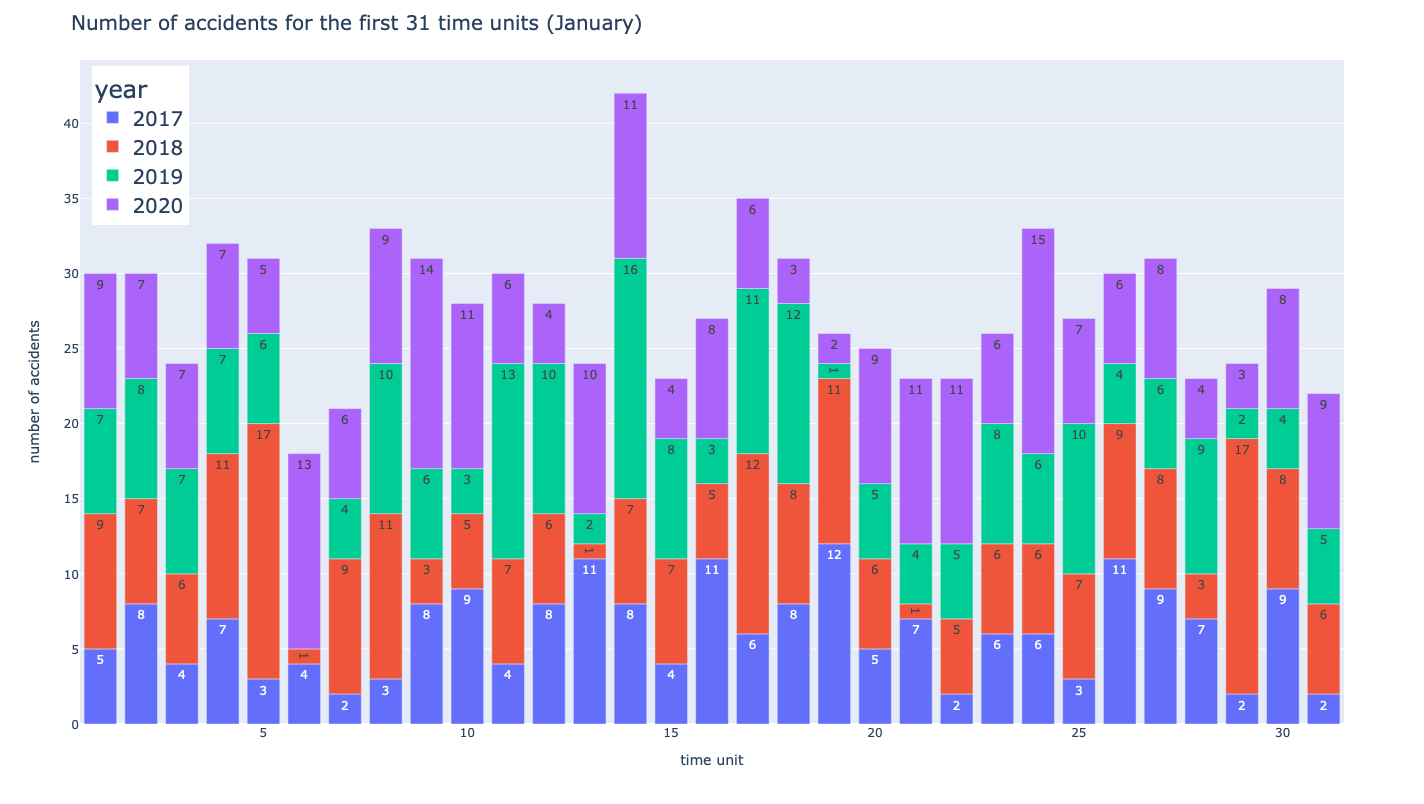
\includegraphics[width=13.5cm]{images/stackedBarPlot.png}
    \caption{The daily number of accidents in Lithuania during the month of January for the four years.}
    \label{fig:January}
\end{figure}

The bar plot of Figure \ref{fig:January} shows the number of accidents recorded in Lithuania on a daily basis for the month of January over the four years. As can be seen from the graph, the number of accidents happening highly fluctuates day by day, indicating that the underlying intensity of the Poisson process is dependent on time and makes a strong case for a time in-homogeneous approach. 

The state space of the non-homogeneous Poisson process is denoted by $\mathcal{S}$ and is defined as follows:
\begin{equation}
    \mathcal{S} =  E\cup V_{\cap}
\end{equation}, where
\begin{equation*}
    E = \{e: e\in E(G_0)\}
\end{equation*}
\begin{equation*}
    V_{\cap} = V(G_0) \cap \mathcal{I}
\end{equation*}

In other words, the state space consists of the union of the edges of the road graph and the vertices that represent intersection points of the road network.

\section{Estimating the Cumulative Intensity of a NHPP}
In an attempt to simulate from a non-homogeneous Poisson process where the events of interest have a spatial component, Zhang and Zheng \cite{triangulation} use a triangulation of the state space in order to interpolate a piece-wise linear estimator of the intensity between the triangular regions of the state space partition. However, a triangulation of the state space falls far away from the current framework since it would require a major change of the structure of the state space (which is considered to be a road graph). Leemis \cite{nonparametric} follows a simpler yet powerful strategy that does not depend on the state space of the process and uses a piece-wise linear estimator of the cumulative intensity function to simulate the arrival times of a NHPP by inversion. For this work the latter philosophy is adopted. 
\subsection{Mathematical Background}
In order to estimate the cumulative intensity function of the non-homogeneous Poisson process a non-parametric, piece-wise linear estimator is used to interpolate between the time values. Let $(0,S]$ be the time horizon of the NHPP, where $S$ is a known constant. Under the assumption that the intensity function $\lambda(t)$ is positive and continuous for almost every $t\in(0, S]$ the estimation proceeds as follows:

\begin{definition}[Empirical Cumulative Intensity Function of the NHPP (ECIF)]
    Let $k$ be the number of realisations of the process, $n_i$ for $i=1,...,k$ be the number of observations in the $i^{th}$ realisation and $n$ be the  total number of observations, i.e., $n=\sum_{i=1}^k n_i$. Denote by $t_{(1)}, ...,t_{(n)}$ the order statistics of the arrival times upon superposition of the realisations. Assume that, $t_{(0)}=0$, $t_{(n+1)}=S$ and $\hat{\Lambda}(S)=\frac{n}{k}$.
    
    The empirical cumulative intensity function of the NHPP evaluated on a time value $t$ is defined as:
    \begin{equation}
        \Lambda(t)=\frac{\mathlarger{\sum_{i=0}^{n+1}} \mathbb{I}_{(t_i\leq t_{i+1})} \cdot \mathbb{I}_{(t_{i+1}\leq t)}}{k}
    \end{equation}
    for $k\geq 1$.
    
    In other words, the empirical cumulative intensity function of the NHPP evaluated on a point in time $t$ is the average number of events that have occurred upon the superposition of the realisations. 
\end{definition}

\begin{definition}[Estimator of the Cumulative Intensity Function of the NHPP]
    Let $k$ be the number of realisations of the process, $n_i$ for $i=1,...,k$ be the number of observations in the $i^{th}$ realisation and $n$ be the  total number of observations, i.e., $n=\sum_{i=1}^k n_i$. Denote by $t_{(1)}, ...,t_{(n)}$ the order statistics of the arrival times upon superposition of the realisations. Assume that, $t_{(0)}=0$, $t_{(n+1)}=S$ and $\hat{\Lambda}(S)=\frac{n}{k}$.
    
    The piece-wise linear estimator of the cumulative intensity function $\Lambda(t)$ between the time values $t_{(i)}<t\leq t_{(i+1)}$ for $i=0,...,n$ is defined as:
    \begin{equation}\label{estimator}
    \hat{\Lambda}(t) = \frac{in}{(n+1)k} + \frac{n(t-t_{(i)})}{(n+1)k(t_{(i+1)}-t_{(i)})}.
    \end{equation} 
    
    If for some $m$, $t_{(m)}=t_{(m+j)}$, for $j\geq 1$ i.e., more than one event occurred simultaneously, then $$\hat{\Lambda}(t_{(m)}) = \frac{mn}{(n+1)k}.$$
\end{definition}

\subsection{Implementation}
In order to estimate the cumulative intensity of the NHPP there are two strategies that can be followed based on the assumptions that are made regarding the homogeneity of the process on a yearly basis. Specifically, if the assumption is made that a year is not differentiable by another in terms of the underlying patterns that yield the events, then the four year period of observations can be treated as four realisations of the process, where the time horizon is one year. In that case, $k=4$ and $S=365$.


If the assumption is omitted and each year is considered independently, then the time horizon is four years and more specifically $S=1461(=4\times 365 +1)$. Under this approach, the number of realisations of the process is $k=1$ which consists of all of the available observations ordered in ascending arrival time order. 

\begin{figure}
    \centering
    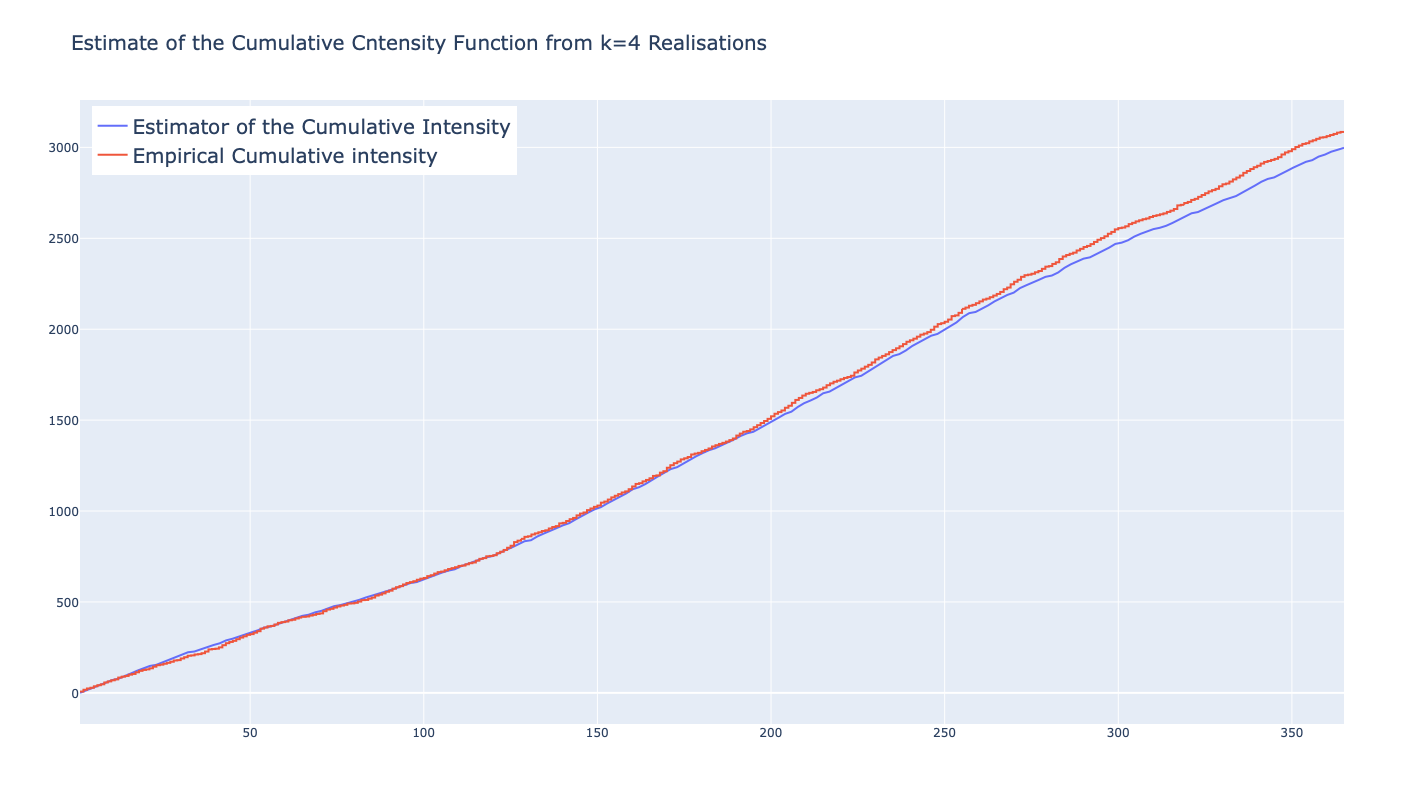
\includegraphics[width=12cm]{images/estimatorKfull.png}
    \caption{Estimate of the cumulative intensity function from $k=4$ realisations of the process over a period of $365$ days.}
    \label{fig:estimatorK}
\end{figure}

The graph of Figure \ref{fig:estimator14} depicts the estimator of the cumulative intensity function evaluated in time values from the interval $(0, 365]$. In addition, the empirical cumulative intensity is evaluated on every integer time unit $0,1,2,...,365$. These units correspond to the ordered days of the one year period and thus the number of accidents that have collectively occurred can be obtained through aggregations.

 \begin{figure}[!ht]
    \centering
    \subfloat[\centering $k=1$ realisation ]{{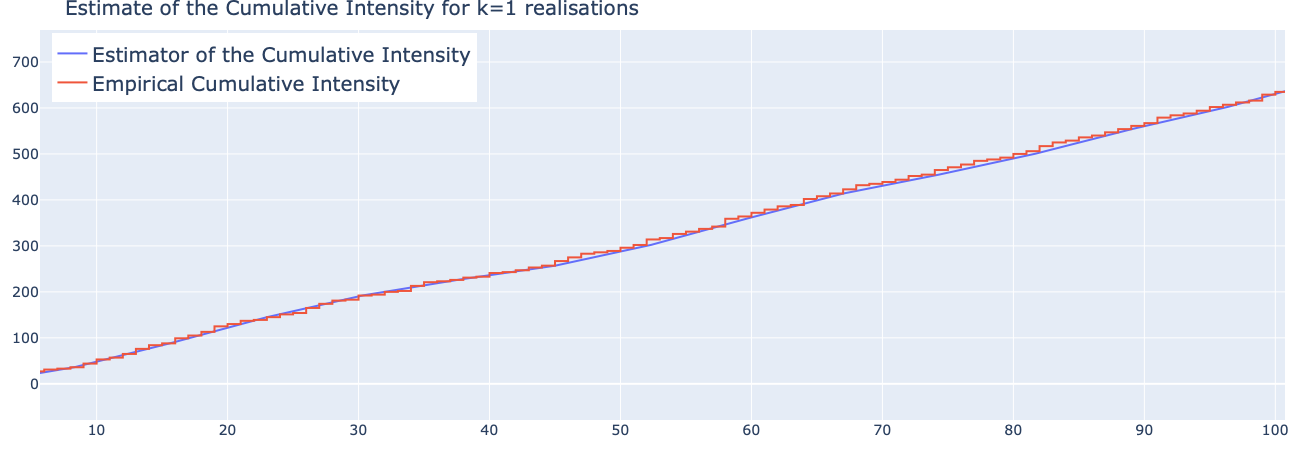
\includegraphics[width=12cm]{images/estimatorK1_100.png} }}%
    \qquad
    \subfloat[\centering $k=4$ realisations  ]{{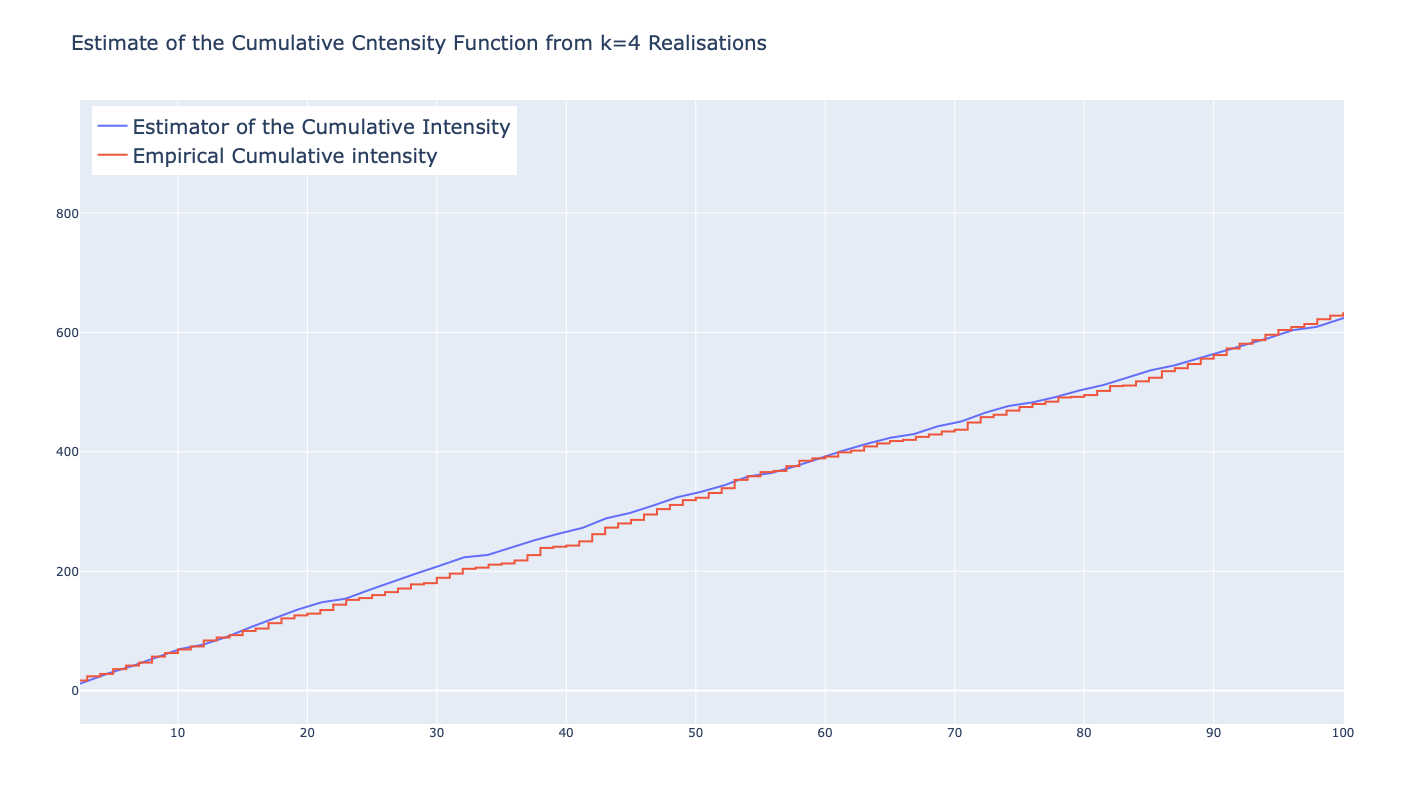
\includegraphics[width=12cm]{images/estimatorsK_100.png} }}%
    \caption{The piece-wise linear estimator of the cumulative intensity function for the first $100$ units of the time horizon. (a) The estimator is obtained from $k=1$ realisations of the process over a period of $4$ years ($1461$ time units). (b) The estimator is obtained from $k=4$ realisations of the process over a period of $1$ year ($365$ time units).}%
    \label{fig:estimator14}
\end{figure}

A comparison between the two possible strategies on the number of realisations of the process can be obtained by the graph of Figure \ref{fig:estimator14}. 
Due to the large number of points and the fact that the estimate is quite close to the empirical cumulative intensity function, the graph is restricted to the first $100$ days of the time horizon for each case, to allow visible inspection of the two curves to some extent. Figure \ref{fig:estimator14} (a) corresponds to the first $100$ days, when the period of the process is $1461$ time units (days) and the number of realisations is $k=1$. The alternative case of $k=4$ realisations over a period of $365$ time units is shown on the sub-plot (b) of the same Figure. 

One important property of the chosen estimator, apart from enabling the estimation of the cumulative function at any time $t\in (0, S]$ is that as a non constant linear function it is subject to inversion. This inversion can be used to simulate the arrival times of the NHPP.

\section{Simulating an NHPP by Inversion}
\subsection{Background}
When it comes to simulating variates from a non-homogeneous Poisson process, there  are three classic methods; inversion, composition and thinning (for details see Devroye \cite{classicsimulation}). Simulating with inversion refers to the actual inversion of the cumulative intensity function and can be troublesome in cases where the intensity function is not invertible. In such cases, numerical approximations are put into action with some iterative method. Luckily, in this framework the cumulative intensity function although not subject to inversion itself is estimated by a linear function that can be successfully inverted.

Simulating via composition is implemented in cases where there is a natural decomposition of the analytical form of the intensity function in a sum of $n$ intensities, i.e. $\lambda(t)=\sum_{i=1}^n \lambda_i(t)$. This way, the NHPP of interest is decomposed into $n$ sub-processes. Each of these $n$ sub-processes is simulated and the sequence of the ordered variates is a variate of the initial process. Intuitively, the composition method is justified by the independent number of arrivals of Poisson processes for disjoint intervals and the following fundamental property of the Poisson distribution (for the proof see \cite{ross}):

If $X_1,..., X_n$ are independent Poisson distributed random variables with parameters $\lambda_1,..., \lambda_n$ respectively, then the random variable $X=\sum_{i=1}^n X_i$ is Poisson distributed with parameter $\lambda=\sum_{i=1}^n \lambda_i$. 

Lastly, the third of the classic Poisson process variate generation methods, thinning, provides a way to simulate a NHPP through the simulation of a homogeneous Poisson process whose intensity $\mu(t)$ is an upper bound of the intensity $\lambda(t)\hspace{0.2cm}\forall t$. In this case, variates from the homogeneous Poisson process with rate $\mu(t)$ are obtained via inversion and each variate is rejected with probability $1-\frac{\lambda(t)}{\mu(t)}$. Note, that the closest the dominating intensity $\mu(t)$ is to $\lambda(t)$ more variates are accepted under the NHPP. 

\subsection{Implementation}
To generate variates of arrival times for the non-homogeneous Poisson process, the estimator in \eqref{estimator} is used by means of inversion as can be seen in Algorithm \ref{alg:simulation}. The intuition behind inversion and Algorithm \ref{alg:simulation} lies in the distribution of the arrival times. 

Let $0<T_1<T_2,...$ be the arrival times of a NHPP in increasing order of occurrence. Then, given $T_n=t$ for some $n\in\mathbb{N}$, and $x\geq 0,$ $$F(x)=P(T_{n+1}-T_n>x|T_n=t)=P(N(t, t+x)=0|T_n=t)=e^{-(\Lambda(t+x)-\Lambda(t))}.$$ In other words, $T_{n+1}-T_n$ is distributed according to $$F(x)=1-e^{-(\Lambda(t+x)-\Lambda(t))}.$$ As a result, $T_{n+1}$ is distributed as $T_n + F^{-1}(U)$, where $U$ is a uniform random variable. By expressing $U$ as $1-e^{-E}$, where $E$ is an exponential random variable, the distribution of $T_{n+1}$ can be written as $\Lambda^{-1}(E+\Lambda(T_n))$ \cite{classicsimulation}. In addition, the event times of a NHPP can be obtained by the event times of a homogeneous Poisson process by the transformation $T_i=\Lambda^{-1}(E_i)$ \cite{cinclar}. By substituting the cumulative intensity function with the piece-wise linear estimator given in \eqref{estimator}, one can obtain a closed form for the $i^{th}$ arrival of the NHPP. 
\begin{equation}\label{inverted}
\begin{aligned}
    \hat{\Lambda}(t) = u\Rightarrow 
    \frac{in}{(n+1)k} + \frac{n(t-t_{(i)})}{(n+1)k(t_{(i+1)}-t_{(i)})}=u\\
    t =\left ( \frac{uk(n+1)}{n}\right )(t_{(i+1)}-t_{(i)}) -i (t_{(i+1)}-t_{(i)}) + t_{(i)} \Rightarrow\\
    \hat{\Lambda}^{-1}(u) = t_{(i)} + \left [\frac{u(n+1)k}{n} - i \right ](t_{(i+1)}-t_{(i)}) 
\end{aligned}
\end{equation}
Evaluating equation \eqref{inverted} on an arrival time $E_m$ of a homogeneous Poisson process for some $m$ gives, 
\begin{equation}
    \hat{\Lambda}^{-1}(E_{(m)}) =  t_{(m)} + (t_{(m+1)}-t_{(m)})\left [\frac{E_{(m)}k(n+1)}{n}-m\right ]
\end{equation}

\begin{algorithm}
  \caption{Simulation of the arrival times of a NHPP}
  \label{alg:simulation}
  \begin{algorithmic}
    \State{\textbf{Input: }$n$-number of observations, $k$-number of realisations, $\hat{\Lambda}$-estimator of the cumulative intensity function}
    \State{$i\gets1$}
    \State{$u\gets \mathcal{U}(0,1)$}
    \Comment{Sample from the Uniform distribution}
    \State{$E_i\gets -log(1-u)$}
    \Comment{Exponential sample}
    \While{$E_i<\frac{n}{k}$}
        \State{$m\gets \floor*{\frac{(n+1)k}{n}E_i}$}
        \State{$T_{(m)}\gets t_{(m)} + [t_{(m+1)}-t_{(m)}]\left(\frac{(n+1)k}{n}E_i-m \right)$}
        \Comment{Inversion step}
        \State{$i\gets i+1$}
        \State{$u\gets \mathcal{U}(0,1)$}
        \State{$E_i\gets E_{i-1} - \log(1-u)$}
    \EndWhile
    \State{\textbf{Output: }Arrival times of $i$ events of a NHPP}
  \end{algorithmic}
\end{algorithm}

\begin{figure}
    \centering
    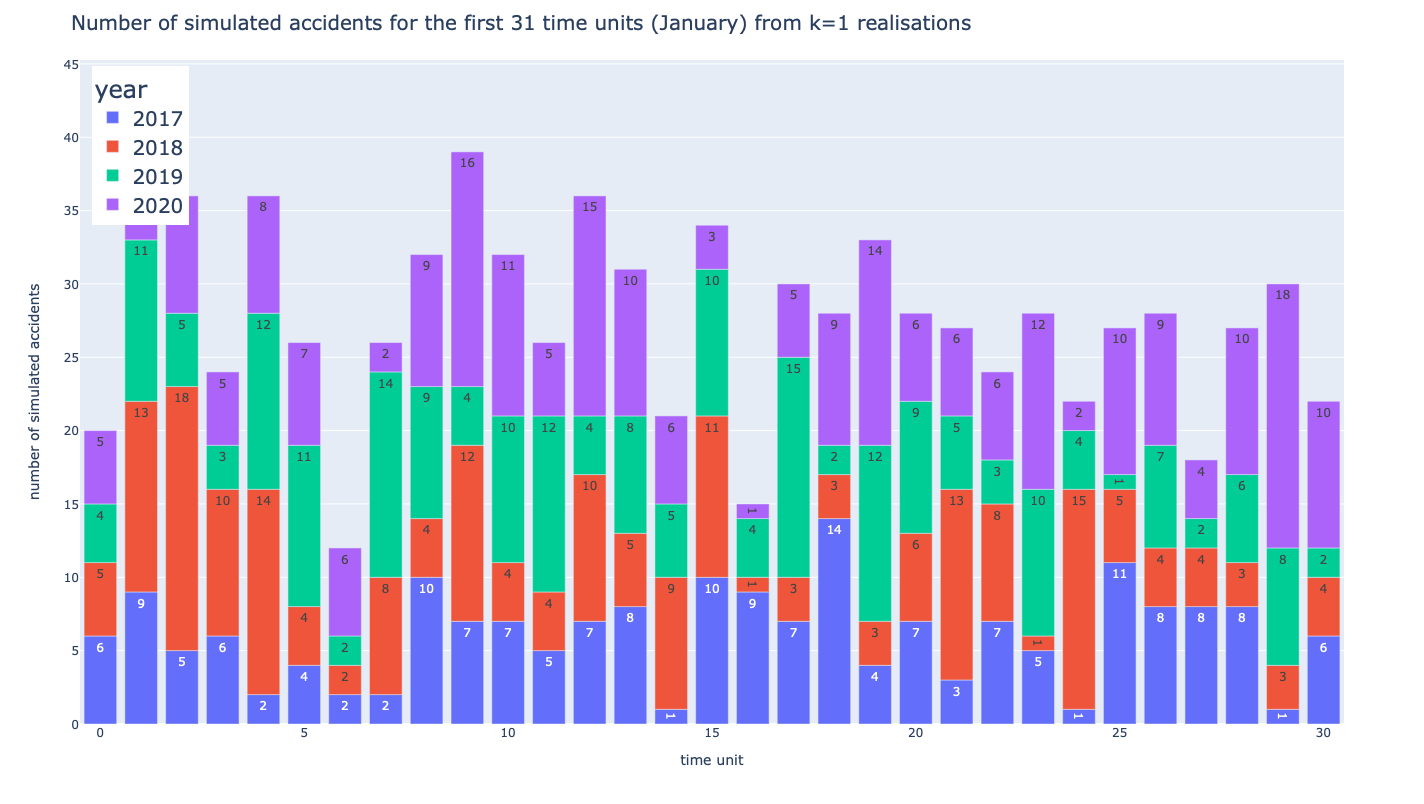
\includegraphics[width=13.5cm]{images/simulation_result_1.png}
    \caption{The daily simulated number of accidents in Lithuania during the month of January for the four years.}
    \label{fig:JanuarySimulation}
\end{figure}


As previously mentioned, the lowest time resolution of interest is the day of the year and thus the generated variates are rounded into the day that they belong to. This way, each day of the four year period is associated with a number of simulated events. 

Figure \ref{fig:JanuarySimulation} illustrates the number of simulated events from Algorithm \ref{alg:simulation} for the first $31$ time units of each year from $k=1$ realisations of the NHPP.

The next step is to associate these events in terms of their geographic position and specifically in their position in the road graph $G_0$. Taking into account that the state space of the Poisson process under question consists of the union of the intersection vertices and the edges of the road graph, each event shall be mapped into one element of the state space or in other words one element of road graph that is also a member of the state space. This can be done by sampling from the distribution of the state space, i.e. the distribution of intersections and edges. While the true distribution of the states is unknown, one can estimate it by the locations of accidents in the provided dataset combined with the map-matching algorithm. This way, each state after observing the data has a known number of events falling on it. 

One way to consider each state in the state space is as a categorical variable. From such a viewpoint, the $n$ events of the Poisson process can be seen as $n$ independent trials, where each trial results in one of the states. The following section exploits this intuition and provides the necessary mathematical framework to model the state counts and estimate the conditional distribution of the state space. 

\subsection{Modelling counts}
\subsubsection{Dirichlet Multinomial conjugate priors}
The multinomial distribution is a generalisation of the binomial distribution and it is often used to model counts of events. For example, consider a $k$-sided die that is rolled independently $n$ times. Then the probability of the count for each side can be modelled by the multinomial distribution.  

\begin{definition}[Multinomial Distribution]
    Let $k\in \mathbb{N}$ be the number of possible, mutually exclusive outcomes, over $n$ independent trials and let $p_i$ for $i=1,...,k$ be the probability of outcome $i$. Then, $p_i\geq 0, \forall i\in \{1,...,k\}$ and $\sum_{i=1}^k p_i=1$. Denote by $X_i$ the number of times outcome $i$ is observed over the $n$ trials. Then, the random vector $\Vec{X}=(X_1,...,X_k)$ is said to be distributed according to the multinomial distribution with parameters $n$ and $\Vec{p}=(p_1,...,p_k)$. 
\end{definition}  

What is worth mentioning is that, despite the $n$ trials conducted independently, the outcomes $X_i$ for $i=1,...,k$ are not independent since the sum of them should be equal to $n$. 

\begin{corollary}[Probability Mass Function of the Multinomial Distribution]
    Let $\Vec{X}=(X_1,...,X_k)$ be a random variable with multinomial distribution with parameters $n,p_1,...,p_k$, i.e. $\Vec{X}\sim Multinomial(n,p_1,...,p_k)$.

    Then, the probability of $(X_1=x_1,...,X_k=x_k)$ for some $x_i,\hspace{0.2cm} i=1,...,k$, or in other words the probability mass function is given by
    \begin{equation}\label{MultinomialDensity}
        f(x_1,...,x_k;n,p_1,...,p_k)
        =\frac{n!}{x_1!...x_k!}p_1^{x_1}\times...\times p_k^{x_k},
    \end{equation} where $n=\sum_{i=1}^k x_i$ and $0$ otherwise. 

\end{corollary}

The probability mass function in \eqref{MultinomialDensity} can be rewritten by using the following property of the Gamma function:
\begin{equation*}
    \Gamma(n)=(n-1)!,\hspace{0.2cm} n\in\mathbb{Z}.
\end{equation*} Thus, replacing the factorials in \eqref{MultinomialDensity} with the equivalent Gamma expression, the probability mass function is 
\begin{equation}
    f(x_1,...,x_k;n,p_1,...,p_k)=\frac{\Gamma(\sum_{i=1}^k x_i +1)}{\prod_{i=1}^k\Gamma(x_i+1)}\prod_{i=1}^k p_i^{x_i}.
\end{equation}

\subsubsection{Simulating Locations from the Conditional Distribution of States}
In order to estimate the state intensity of the non-homogeneous Poisson process the multinomial distribution is used to model the per state count of occurring events for a given day. In addition, a non informative prior is used to encode the probability of one event occurring in one state before any accident is observed. In Bayesian statistics, the Dirichlet distribution is often used as a prior and in this case there might not be a distribution more appropriate since the Dirichlet is in fact the conjugate prior of the Multinomial distribution. 

\begin{definition}[Probability Density Function of the Dirichlet Distribution]
    Let $k\geq 2, k\in \mathbb{N}$ and $\alpha_1,...,\alpha_k>0$. Then, the Dirichlet distribution with parameters $\alpha_1,...,\alpha_k$ has the following probability density function \footnote{with respect to the Lebesgue measure}:
    \begin{equation}\label{DirichletDensity}
    f(x_1,...,x_k;\alpha_1,...,\alpha_k)=\frac{\Gamma(\sum_{i=1}^k \alpha_i)}{\prod_{i=1}^k\Gamma(\alpha_i)}\prod_{i=1}^k x_i^{\alpha_i-1}
    \end{equation}, where $\sum_{i=1}^kx_i=1$ and $x_i\geq 0\hspace{0.2cm}\forall i\in\{1,...,k\}$   
\end{definition}
 
Note that the support of the Dirichlet distribution can be interpreted as the set of $k-$ dimensional discrete probability distributions. 

In the case where the parameters $a_1,...,a_k$ have equal values the Dirichlet distribution is characterised as symmetric. The symmetric Dirichlet distribution can be used as a non informative prior distribution in cases where the prior knowledge does not favour any component. 

\begin{corollary}[The Dirichlet distribution is the conjugate prior of the Multinomial distribution]
\end{corollary}

Let
\begin{equation*}
    \begin{aligned}
    y_1,...,y_k \sim Multinomial(p_1,...,p_k)\\
    \theta = (p_1,...,p_k) \sim Dirichlet(\alpha_1,...,\alpha_k)
    \end{aligned}
\end{equation*} 
Then the posterior
\begin{equation*}
    \begin{aligned}
    f(\theta|D) \propto f(\theta, D)
    =f(p_1,...,p_k|\alpha_1,...,\alpha_k)\prod_{y_i\in D} f(y_i|p_1,...,p_k)\propto \\
    \propto \prod_{j=1}^k p_j^{a_j-1}\prod_{y_i\in D}\prod_{j=1}^k p_j^{\mathbb{I}(y_i=j)}
    =\prod_{j=1}^k p_j^{\alpha_j -1 + \sum_{y_i\in D}\mathbb{I}(y_i =j)}
    =Dirichlet(a_j')
    \end{aligned}
\end{equation*}, where $a_j'=a_j + c_j$ and $c_j=\#\{y_i = j\}$ for $j=1,...,k$. 

In addition, the posterior mean is 
\begin{equation*}
    E[y_j] = \frac{a_j'}{\sum_{i=1}^k a_i'}
\end{equation*}

Taking into account that the data consists of a set of states and a number of events falling in those states at a given point in time (specifically, a given day of the period), the focus is shifting to the posterior distribution of the states given a point in time after observing the available data. This way, for each desired time unit (i.e. for each day), the posterior distribution of the states given a time unit (day) is obtained. Having established that, for each arrival time of the process simulated in Algorithm \ref{alg:simulation}, a state to associate that arrival time with is sampled.

\begin{algorithm}
  \caption{Simulating the location of an event in a NHPP}
  \label{alg:SimulateLocation}
  \begin{algorithmic}
    \State{\textbf{Input: }The conditional (posterior) distribution of states $F$ given the arrival time $t$}
    \State{$U\gets \mathcal{U}(0,1)$}
    \Comment{Uniform sample}
    \State{$state\gets F^{-1}(U)$}
    \Comment{Sample from the posterior distribution of states}
    \State{$sample\gets state$}
    \State{\textbf{return: }$sample$}
    \State{\textbf{Output: }An element of the underlying road graph (edge of vertex)}
  \end{algorithmic}
\end{algorithm}

Algorithm \ref{alg:SimulateLocation} contributes towards the simulation of the location for a given arrival time generated by Algorithm \ref{alg:simulation}. 


 \begin{figure}[!ht]
    \centering
    \subfloat[\centering  ]{{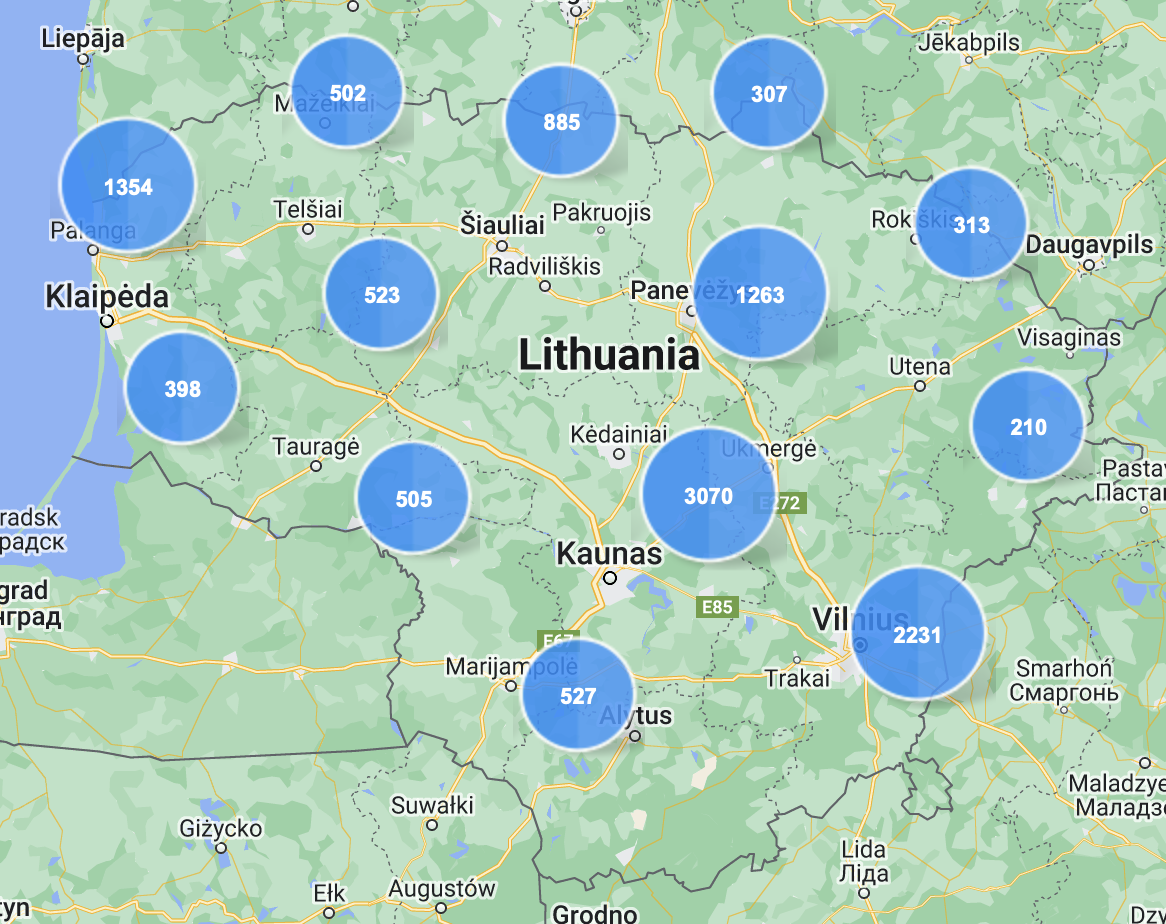
\includegraphics[width=9cm]{images/bubbles.png} }}%
    \qquad
    \subfloat[\centering   ]{{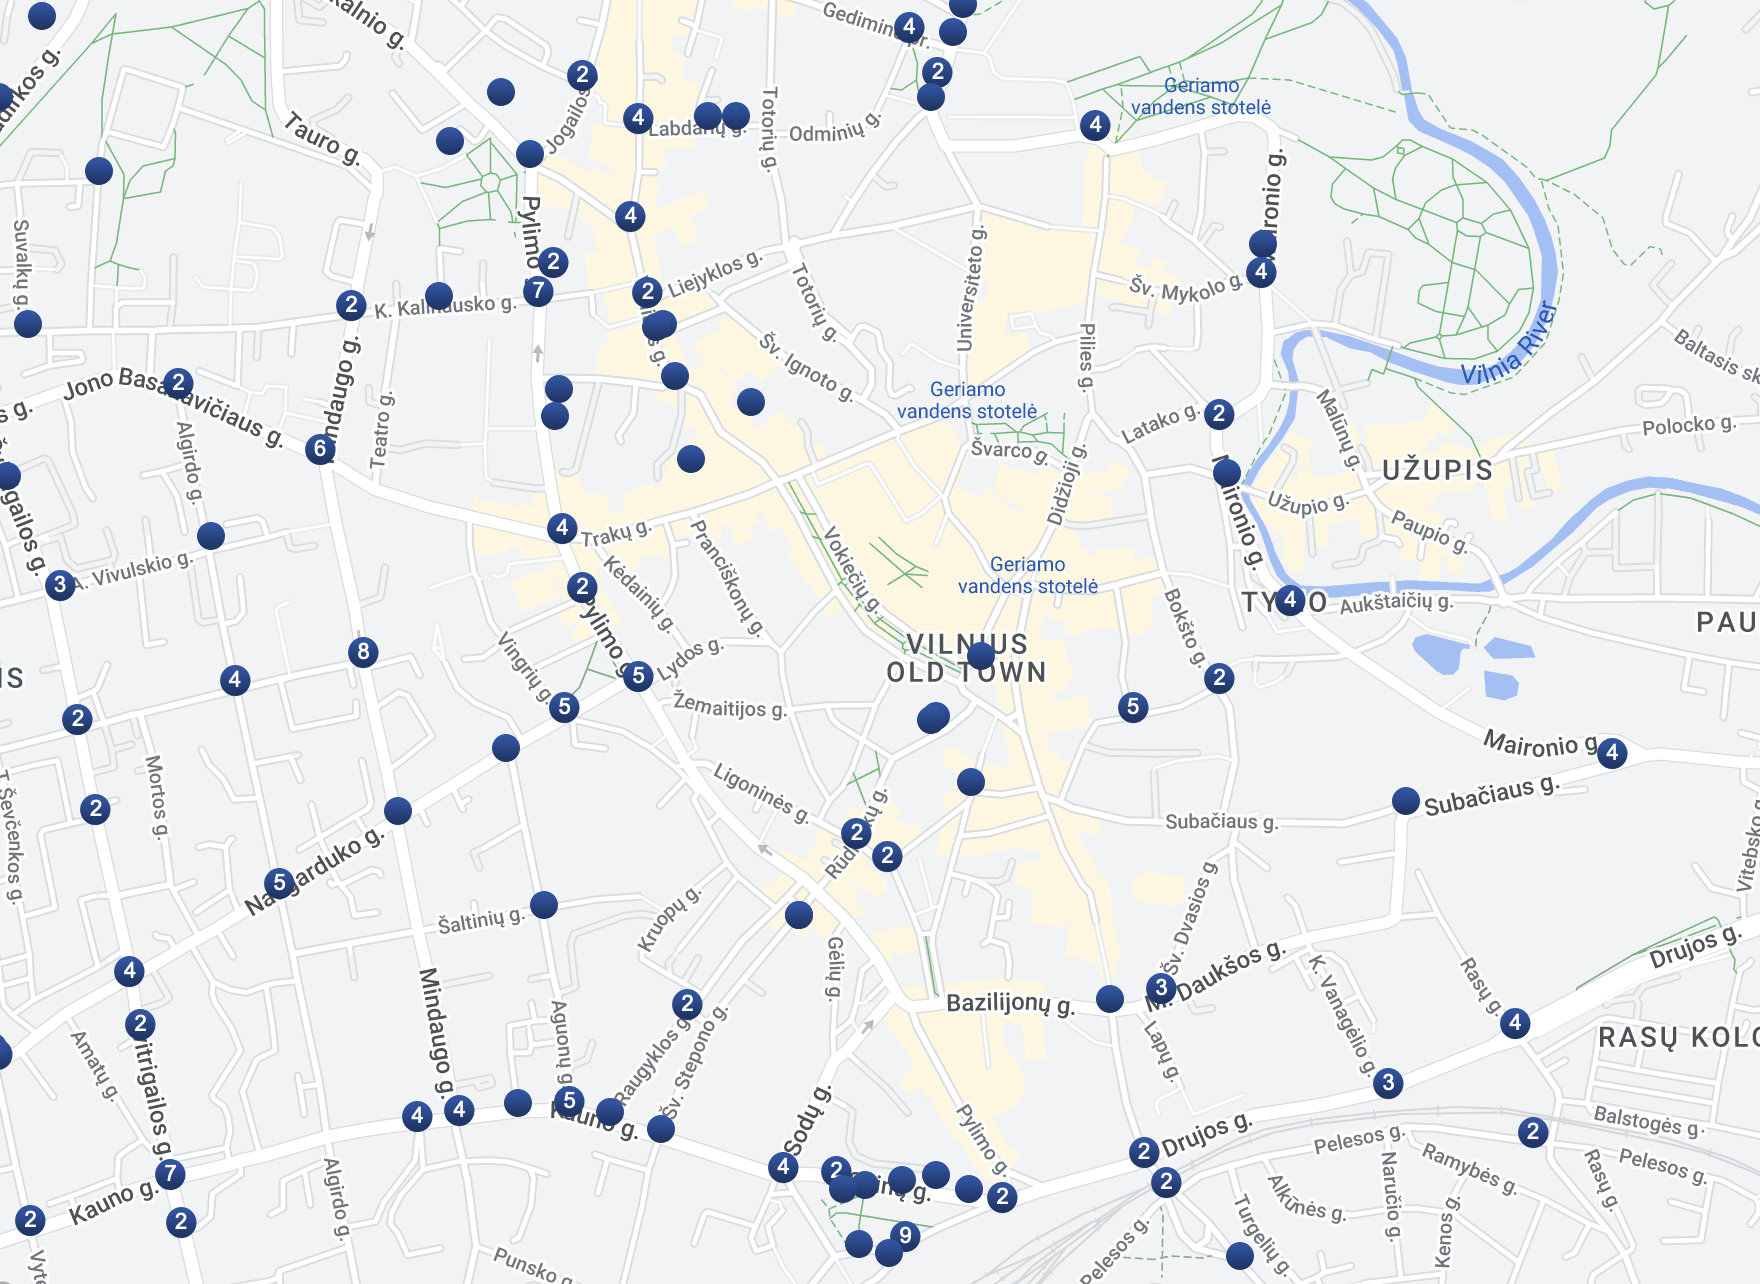
\includegraphics[width=9cm]{images/bluepoints.png} }}%
    \caption{The result of the simulation in terms of spatial position. (a) The number of generated samples aggregated by proximity. (b) The location of the generated samples for a small area in Vilnius. Each variates' location is represented by a blue sphere where the assigned number represents the number of events corresponding to that position. An unlabelled sphere is assumed to represent a single generated event.}%
    \label{fig:result}
\end{figure}

Finally, the result of the simulation in terms of the location of the generated variates is shown in Figure \ref{fig:result}. Figure \ref{fig:result} (a) illustrates the number of simulated events aggregated by proximity at a low resolution, covering all of Lithuania. Subplot (b) of the same Figure depicts the locations of a subset from the generated events on a small central area in the capital Vilnius.  

\section{Environment Configuration and Scalability Discussion}
The framework is implemented within the Apache Spark Ecosystem in a cluster where the maximum number of compute nodes is $8$, each with $16$ GB of memory and $4$ cores. All of the necessary computations and queries were programmed in the programming language Scala, except for those relevant to visualisation purposes where Python was used. The choice of Scala as the primarily used programming language for this work is justified by the big volume of data that were to be processed for the construction of the road graph and its subsequent queries and analytical tasks. More analytically, Scala is the language in which Spark is built in and thus by using Spark's native language the optimisation in terms of efficiency of computations is maximised. 

Regarding the ability of the application to scale onto datasets of arbitrarily large volume, it is theoretically possible to do so by simply increasing the number of compute nodes. The reason behind this, is the extensive use of Spark's Dataframes throughout the majority of the implementation in combination with the use of Spark's built-in functions to the largest extent possible. This results in a very high level of optimisation; which is in practice established through the fact that even though sometimes the computations include million of records at a time, the run-time for those computations is a couple of seconds long. Throughout all of the stages of processing, only one of them takes significantly more time to be completed and that refers to the sampling from the conditional distribution of states described in Algorithm \ref{alg:SimulateLocation}. Behind this there are two aspects; one of them refers to I/O bound time connected to identifying the right file containing the conditional distribution for the day at hand and loading it, and the other one to the actual sampling from the distribution. Having said that, the run time for that task is not significantly affected by obtaining a larger number of samples. 

\section{Summary}
This project presents a method for the construction of a road graph from a road network consisting of open source spatial data. An extension of the method is provided that allows for control of the segmentation level of the network and consequently of the graph, based on an approximation of the geodesic distance between two intersection points of the network. Furthermore, a solution for associating points of the road network that do not necessarily belong to one of the elements of the road graph to their geographically nearest vertex or edge. This is done by extending the highly efficient map-matching algorithm from the GeoMatch project to relate a set of points to a set of graph elements. Apart from the implementation details of these steps that are of great interest on their own due to the large volume of data that is processed concurrently, the previously mentioned stages prepare the scene for modelling a point process whose state space is a sub-set of a road graph's elements.

In order to simulate vehicle collisions happening on a road graph over a period of time, an underlying Poisson point process is assumed. The state space of the process is defined to be a subset of the vertices of the graph together with the set of the graph's edges. Taking into account that the number of accidents happening fluctuates significantly over time the non-homogeneous Poisson process is more appropriate in order to model the arrival times of the events. Thus, the latter is used in an attempt to capture the underlying spatio-temporal patterns that yield the arrivals and to allow the generation of variates. A non-parametric piece-wise linear function estimates the cumulative intensity function of the process from one or more realisations and its inversion is used to generate the arrival times. The next step is to locate the variates in terms of their position in the state space of the road graph.

Simulating the location of the generated times of the process is done by sampling from the discrete distribution of the states. This distribution is modelled by the multinomial distribution, as each state can be considered as a category associated with a number of counts throughout a series of independent experiments. This way, generating locations for a given time is equivalent to sampling from the conditional distribution of states given that time. The conditional distribution of states is obtained by estimating the posterior conditional distribution of the states given the available observations and a non informative prior, within a Bayesian framework. 

\section{Conclusions and Future Work}
This attempt to build a scalable framework for simulating a point process on a graph structure is divided into two main stages. The first one focuses on the construction of the graph and the association of the events of the process with elements of the graph. The second stage is concerned with the generation of variates of the process, which is in turn divided into two levels; the generation of the arrival time and in sequence the sampling of a state to be assigned to the arrival time. The framework, is implemented into a very large state space and the results in terms of run-time are a promising sign in terms of the ability to scale into even larger state spaces. 
Future work shall revolve around data fusion of attributes relevant to vehicle collisions such as the weather and light conditions. Under this approach, the point process should be generalised into a marked point process. In addition to that, it would be of interest to perform different aggregations to the time that the available accidents take place, such as the day of the week or the time of the day. This way, the period of the process should be adapted accordingly to one week for example or to one day. In such cases, it would be fruitful to establish possible patterns regarding for example a specific day of the week or an hour of the day. 

With this project, the stage is set in order to simulate the arrivals of a point process whose events fall into a graph structure. The main focus of the project does not lie in the simulation result itself, but rather on the tools and techniques necessary to do so in a scalable manner. It would be of great potential for future research to exploit the proposed framework into more complex models and establish the true scalability of the application under those premises. 

\section{Acknowledgements}
All of the code produced for this work is available in the following repository \url{https://github.com/lamastex/working-manuscript-privacyTrajectories/StavroulaVlachouMscThesis} in notebooks. The files necessary to produce the GeoMatch library used in Section \ref{MapMatchingPointsOnARoadGraph} can be found in the following GitHub repository \href{https://github.com/StavroulaVlachou/GeoMatch}{StavroulaVlachou/GeoMatch}.

The relevant code implemented for the data pre-processing of Section \ref{ingestion} and the construction of the road graphs described in Section \ref{RoadGraph}, was written in collaboration with the fellow student Virginia Jimenez Mohedano. 

Map data is copyrighted by  OpenStreetMap contributors and available from \href{https://www.openstreetmap.org}{OpenStreetMap}

This project was supported by {\em SENSMETRY} through a {\em Data Science Project Internship} between 2022-01-17 and 2022-06-05 to Stavroula Rafailia Vlachou and {\em Databricks University Alliance} with infrastructure credits from {\em AWS} to Raazesh Sainudiin, Department of Mathematics, Uppsala University, Sweden.


\section{Literature References}
\bibliographystyle{unsrt}
\bibliography{references.bib}
\end{document}

%%% Local Variables:
%%% mode: latex
%%% TeX-master: t
%%% End:
